\chapter{Gumulscy z~Rudzienka, Zamienia i~Grzebowilka}

% Przednia okładka podrozdziału
\includepdf{Rudzienko_mapa_fin.png}

\section{Rudzienko: 1810~r. - 1820~r.}

Wieś Rudzienko na początku XIX~wieku znajdowała się na terenie zaboru 
austriackiego, następnie w~1809~roku została włączona do Księstwa 
Warszawskiego a~w~1815~roku do Królestwa Polskiego. Do momentu utraty przez 
Polskę niepodległości była częścią ziemi czerskiej województwa mazowieckiego. 
Najbliższymi dużymi ośrodkami miejskimi dla Rudzienka były: oddalona o~około 
pięć kilometrów na południowy zachód Kołbiel oraz oddalony o~około 
10~kilometrów na północny wschód Mińsk Mazowiecki. Rudzienko należało 
w~tamtym czasie do parafii pod wezwaniem Świętej Trójcy w~Kołbieli. Najstarsza  
znana wzmianka o~Rudzienku pochodzi z~1408~roku z~księgi sądowej ziemi 
czerskiej \cite{lzugaj}, gdzie wspomina się o~rycerzu Stanisławie Golibku 
z~Małego Rudna \cite{jlubomirski} (łac. \emph{Stanislaus Golibek de Male 
Ruthna}) - patrz ryc. \ref{fig:rudzienko_1408}. Na początku XIX~wieku 
Rudzienko było częścią pokaźnego majątku chorążego warszawskiego Marcina 
Chrzanowskiego z~Chrzanowa Wielkiego i~Małego (herbu Korab), który 
w~1791~roku nabył majątek Rudno wraz z~przyległościami \cite{dzagorski}. Co 
ciekawe, przez Rudzienko przepływa rzeka Świder, jedna z~najdłuższych rzek 
Mazowsza, której źródła znajdują się na Wysoczyźnie Żelechowskiej w~okolicach 
wsi Wnętrzne i~Mysłów, podobnie jak źródła rodziny Gomulskich.

\begin{figure}[!ht]
    \vspace*{0.5cm}
    \centering 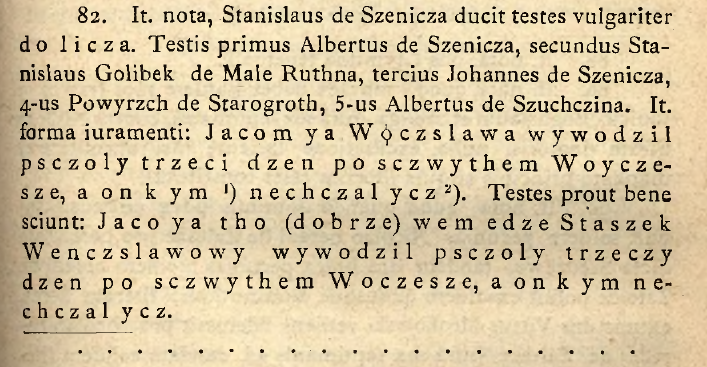
\includegraphics[width=1.0\linewidth]{Rudzienko_1408.png}
    \captionsetup{format=hang}
    \caption{Wpis dotyczący rycerza Stanisława Golibka z~Małego Rudna 
    pochodzący z~księgi sądowej ziemi czerskiej z~1408~roku 
    \cite{jlubomirski}.}
    \label{fig:rudzienko_1408}
\end{figure}

Dnia 12 lutego 1814 roku w~Kołbieli Jan Gomoła ożenił sie z~Łucją Rokicką. 
Wśród skanów akt małżeństw parafii Kołbiel nie zachował się niestety akt 
ślubu Jana i~Łucji, a~przynajmniej nie znajduje się on ani wśród skanów 
dostępnych na portalu \emph{szukajwarchiwach.gov.pl}\footnote{Akta metrykalne 
parafii Kołbiel z~lat 1810-1914 dostępne są pod adresami: \\ 
\url{https://www.szukajwarchiwach.gov.pl/en/zespol/-/zespol/56757} (dostęp: 
marzec 2024 r.)\\ 
\url{https://www.szukajwarchiwach.gov.pl/en/zespol/-/zespol/56631}(dostęp: 
marzec 2024 r.).} ani wśród dokumentów dostępnych w~Archiwum 
Diecezjalnego Warszawsko-Praskiego. W~dostępnych aktach metrykalnych parafii 
pod wezwaniem Świętej Trójcy w~Kołbieli z~roku 1814~można odnaleźć wprawdzie 
13~aktów ślubów, ale nie ma wśród nich aktu ślubu Jana i~Łucji. Skąd w~takim 
razie wiadomo, iż ślub Jana Gomoły i~Łucji Rokickiej w~ogóle się odbył i~że 
miało to miejsce dokładnie 12~lutego 1814~roku? W~Archiwum Diecezjalnym 
Warszawsko-Praskim poza skanami wpisów w~księgach metrykalnych z~parafii 
w~Kołbieli znajdują się również skany indeksów metrykalnych (spisanych po 
łacinie), informujących o~chrzcinach, małżeństwach oraz śmierciach w~tej 
parafii, podzielonych na poszczególne miejscowości, z~których pochodziły 
osoby, których te wpisy dotyczyły. I~właśnie wśród tych indeksów, dla 
1814~roku i~wsi Rudzienko odnaleźć można interesujący nas wpis - patrz ryc. 
\ref{fig:jgomola_1814}.

\begin{figure}[!ht]
    \vspace*{0.5cm}
    \centering 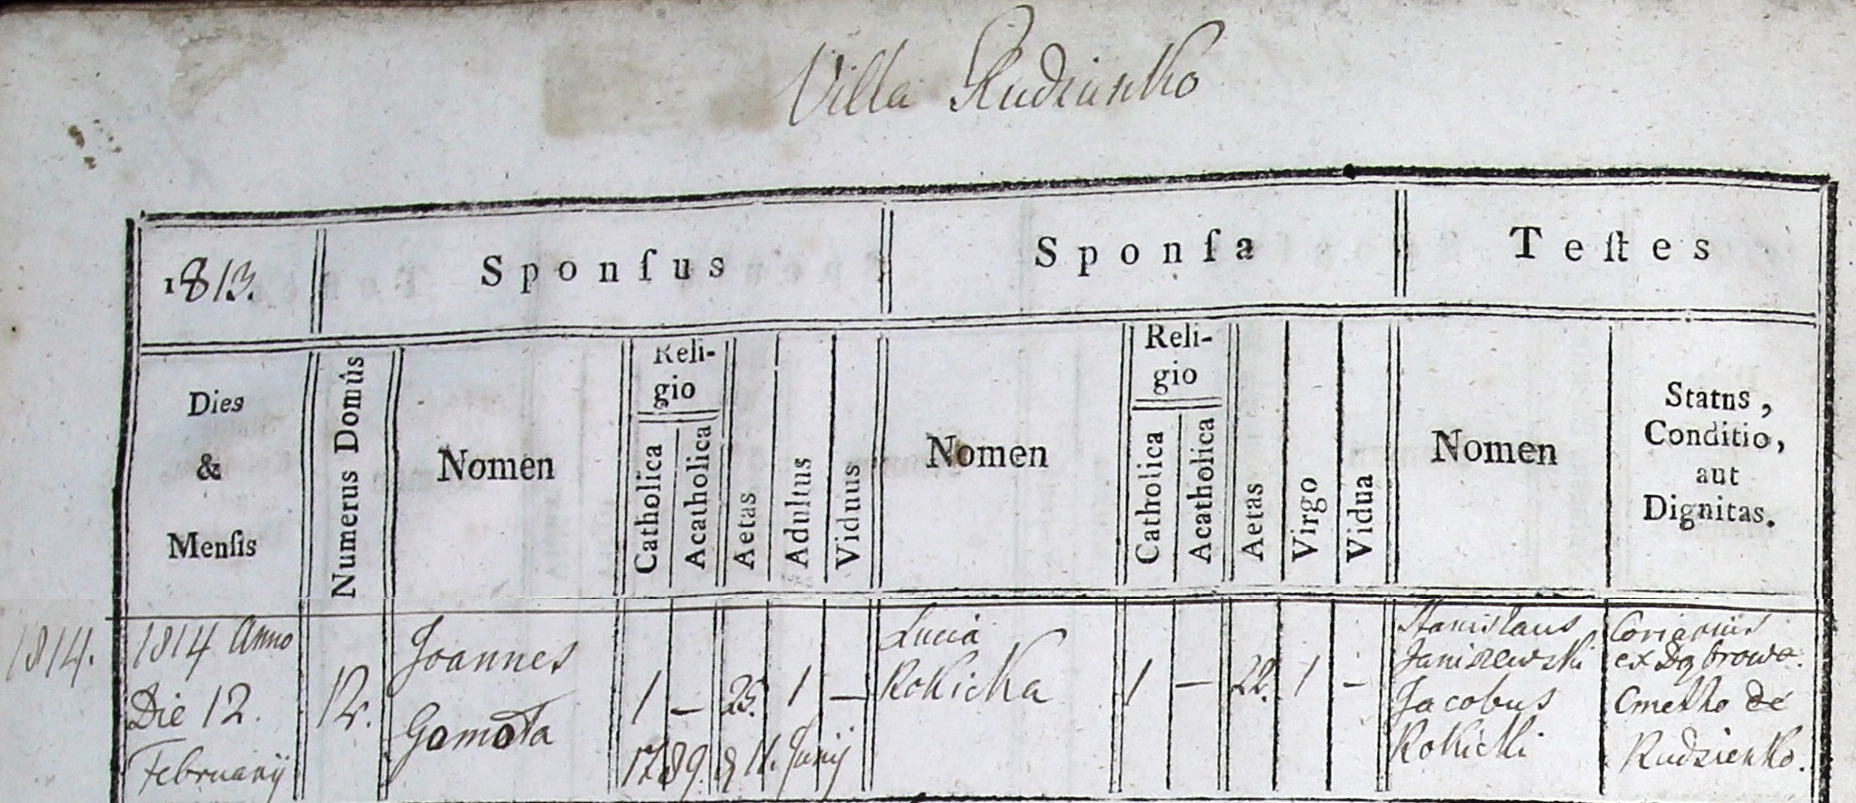
\includegraphics[width=1.0\linewidth]{
        1814_Jan_Gomoła_Łucja_Rokicka_akt_ślubu_parafia_Kołbiel_wpis_NN.png}
    \captionsetup{format=hang}
    \caption{Wpis dotyczący ślubu Jana Gomoły i~Łucji Rokickiej z~1814~roku 
    w~parafii pod wezwaniem Świętej Trójcy w~Kołbieli \cite{par_kolbiel1}.}
    \label{fig:jgomola_1814}
\end{figure}

Z~wyżej wskazanego wpisu jasno wynika, iż Jan Gomoła (łac. \enquote{Joannes 
Gomoła}) urodzony 11~czerwca 1789~roku\footnote{Co w~stu procentach pokrywa 
się z~datą urodzenia Jana Gomoły z~Mysłowa - patrz ryc. 
\ref{fig:gomola3_lubgens}} (łac. \enquote{1789~11.~Junij}) wziął ślub dnia 
12~lutego 1814~roku (łac. \enquote{1814~anno Die 12.~Februarij}) z~Łucją 
Rokicką (łac. \enquote{Lucia Rokicka}), lat 22, a~świadkami tego ślubu byli 
Stanisław Janiszewski oraz Jakub Rokicki. Pozostaje jednak pytanie czemu Jan 
Gomoła z~Mysłowa przeprowadził się akurat do oddalonego o~około 50~kilometrów 
Rudzienka, w~sytuacji gdy mobilność ludności chłopskiej na początku XIX~wieku  
była bardzo ograniczona, szczególnie na tak dużych dystansach. Odpowiedź na 
to pytanie można odnaleźć analizując historię związku Tomasza Rzewuskiego 
(herbu Krzywda), chorążego łukowskiego i~właściciela dworu w~Mysłowie 
z~Marianną Młyńską (z~domu Chrzanowską), córką chorążego warszawskiego 
Marcina Chrzanowskiego (herbu Korab), właściciela dworu w~Rudnie. Poniżej 
zaprezentowano fragmenty artykułu Dariusza Zagórskiego pod tytułem 
\enquote{Dom wdów. O~dworku w~Rudzienku i~jego mieszkańcach}, który opisuje 
historię związku państwa Rzewuskich:

\begin{quote}{Dariusz Zagórski \\ \null\hfill \emph{Dom wdów. O~dworku 
    w~Rudzienku i~jego mieszkańcach} \\ \null\hfill 
    \url{http://www.kolbiel.eu/historie/003/index.html} (dostęp: marzec 
    2024~r.)}

\textit{Po śmierci pierwszego męża Marianna powtórnie wychodzi za mąż za 
Tomasza Rzewuskiego, chorążego łukowskiego. Wiadomo na pewno, że mieli oni co 
najmniej dwoje dzieci: Anielę Mariannę Józefę ur. w~1797~r. oraz Stanisława 
Kostkę urodzonego w~1798~r. Co do samego Tomasza Rzewuskiego w~niektórych 
aktach bywa nazywany Michałem Tomaszem, Michałem, a~nawet Antonim jednak nie 
ma obecnie dostępnych dokumentów, w~których on sam by się podpisał. Natomiast 
wydaje się, że Michał Rzewuski rzeczywiście istniał i~był jego bratem, gdyż 
jest podpisany na akcie ślubu jego córki jako jej stryj. Prawdopodobnie 
Tomasz Rzewuski miał również brata Jakuba Rzewuskiego, który z~kolei jest 
wymieniony w~akcie ślubu Stanisława Kostki, także jako jego stryj, co więcej 
z~tytułem \enquote{jaśnie wielmożny}. Na przełomie wieków XVIII i~XIX miało 
to jeszcze znaczenie gdyż tak podkreślano wyższe urodzenie szlachcica 
pochodzącego z~rodów piastujących najwyższe państwowe urzędy. Idąc tym tropem 
i~tropem sukcesji majątków ziemskich można by dojść do dość zaskakujących 
wniosków. Jakub Rzewuski brat Tomasza jest wymieniony w~aktach jako dziedzic 
majątku Kanie pod Rejowcem, natomiast Stanisław Kostka po ojcu odziedziczył 
majątek Mysłów pod Żelechowem. W~przeszłości majątki te, a~także same 
miasteczka Rejowiec i~Żelechów należały do jednej osoby – do hetmana 
wielkiego koronnego Wacława Rzewuskiego, później w~pewnej części również do 
jego potomków.
\\
\\
(...)
\\
\\
Czy Rzewuscy pomieszkiwali czasem w~Rudnie czy Rudzienku? Tego nie można być 
pewnym natomiast można niemal na pewno stwierdzić, że formalnie Rudzienko 
przeszło na własność Marianny z~Chrzanowskich wraz ze śmiercią jej ojca 
Marcina Chrzanowskiego co miało miejsce w~roku 1811. Dlatego myślę, że racje 
mają ci autorzy, którzy twierdzą, że dworek w~Rudzienku nie powstał 
równolegle z~pałacem w Rudnie, a~trochę później. Nie wiemy kiedy zmarł drugi 
mąż Marianny z~Chrzanowskich, Tomasz Rzewuski, ale na pewno miało to miejsce 
przed rokiem 1814~w którym to ślub brała najstarsza córka Marianny, Krystyna 
Anna Młyńska. Już wtedy Rzewuski nie był obecny przy ceremonii, a~jego 
miejsce zajmował Józef Grabowski, przyszły trzeci mąż Marianny 
z~Chrzanowskich.
\\
\\
(...)
\\
\\
I~tak, w~roku 1816, w~Wilczyskach Marianna z~Chrzanowskich wzięła ślub 
z~Józefem Grabowskim, podprefektem powiatu żelechowskiego. Mieszkała wówczas 
w~Mysłowie i~była jak wskazuje akt dożywotnią posesorką tego majątku wraz 
z~przyległościami, co znaczy, że małżonkowie Rzewuscy w~czasie swojego 
małżeństwa uczynili taki zapis. Umowa ta dawała dość mocną pozycję wdowie, 
która w~sprawach zarządzania majątkiem miała niemal takie prawa jakby była 
mężczyzną. Był wszakże jeden warunek – musiała pozostać wdową. Kiedy Marianna 
z~Chrzanowskich wyszła za mąż po raz trzeci to umowa z~drugiego małżeństwa 
przestała obowiązywać. Przez jakiś czas wraz z~nowym mężem nadal mieszkali 
w~Mysłowie, przechodzącym teraz na syna Marianny z~drugiego małżeństwa, 
Stanisława Kostkę Rzewuskiego. Potem mogli zamieszkać w~Warszawie przy ulicy 
Długiej, bo Grabowski wynajmował tam kamienicę pod nr 590~jeszcze w~roku 
1819. Całkiem możliwe jest też, że już wtedy, czyli przed rokiem 1820~podjęto 
decyzję o~budowie dworu w~Rudzienku. Zapis w~księgach hipotecznych wskazuje, 
że Mysłów prawnie przeszedł na Stanisława Kostkę w~październiku 1822~r. co 
można by moim zdaniem interpretować wtedy tak, że prace w~posiadłości 
w~Rudzienku był już na tyle zaawansowane, że Grabowscy mogli tam 
pomieszkiwać.}
\end{quote}

Jak wynika z~przytoczonych powyżej fragmentów, Tomasz Rzewuski wziął ślub 
z~Marianną Młyńską z~Chrzanowskich około 1796~roku. W~1811~roku zmarł ojciec 
Marianny, Marcin Chrzanowski, wtedy też doszło do formalnego połączenia się 
majątków Mysłów (wraz z~przyległościami) oraz Rudno (wraz z~przyległościami) 
pod wspólnym zarządem państwa Rzewuskich. Prawdopodobnie dzięki temu 
połączeniu, Jan Gomoła miał szansę przeprowadzić się do Rudzienka i~mógł się 
tam szkolić w~zawodzie kowala. Czy istotnym w~jego historii był fakt, iż 
Tomasz Rzewuski był chrzestnym ojcem jego brata Wojciecha? Nie możemy być 
tego pewni, na pewno przeprowadzka Jana może być kolejną przesłanką 
wskazującą na pewne powiązanie Gomołów z~Mysłowa z~tamtejszym dworem, a~nawet 
z~jego dziedzicem. Około 1814~roku Tomasz Rzewuski zmarł i~wspólny majątek 
Rzewuskich i~Chrzanowskich stał się wyłączną własnością Marianny Rzewuskiej 
z~Chrzanowskich. W~1816~roku, w~Wilczyskach, Marianna Rzewuska wzięła ślub 
z~Józefem Grabowskim, co oznaczało, iż straciła ona prawo do zarządzania 
majątkiem skupionym wokół dworu w~Mysłowie. Mimo to dwory w~Mysłowie 
i~Rudzienku pozostawały pod jej kontrolą do 1822~roku, kiedy to Stanisław 
Kostka Rzewuski, jej syn ze związku z~Tomaszem Rzewuskim, przejął 
w~posiadanie majątek Mysłów należny mu po zmarłym ojcu. Wtedy też, 
prawdopodobnie około 1820~roku, do Rudzienka przybyli: Anna Gomoła, 
najmłodsza siostra Jana, Krystyna Gomoła, córka Andrzeja i~Agaty Gomołów 
z~Wnętrznego oraz Paweł Sokół, syn Macieja i~Marianny, a~bratanek Petronelli 
Gomoły. Wygląda więc na to, że Jan, Anna, Krystyna i~Paweł wykorzystali około 
dziesięcioletnie okno czasowe, w~czasie którego dwory w~Mysłowie i~Rudzienku 
były zarządzane przez tych samych właścicieli, żeby zmienić miejsce 
zamieszkania i~podjąć sie pracy na dworze Marianny z~Chrzanowskich.

\begin{figure}[!ht]
    \vspace*{0.5cm}
    \centering 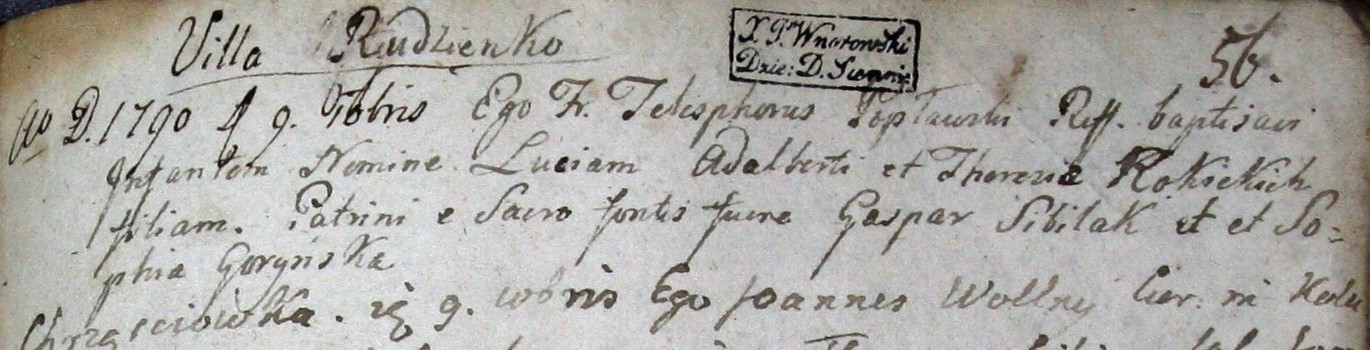
\includegraphics[width=1.0\linewidth]{
        1790_Łucja_Rokicka_akt_chrztu_parafia_Kołbiel_karta_56.jpg}
    \captionsetup{format=hang}
    \caption{Akt chrztu Łucji Rokickiej - par. Kołbiel 1790~rok.}
    \label{fig:lrokicka_1790}
\end{figure}

Tak prawdopodobnie wyglądała historia pojawiania się Gomołów w~Rudzienku na 
początku XIX~wieku. Przechodząc teraz do historii żony Jana Gomoły - Łucji, 
możemy stwierdzić, iż przyszła ona na świat 9~października 1790~roku 
w~Rudzienku (patrz: ryc. \ref{fig:lrokicka_1790}), jako córka Wojciecha 
(ur. 1744~r. - zm. 1834~r.) i~Teresy (ur. 1747~r. - zm. 1836~r.) z~domu 
Skocek. Pochodziła ona z~licznej w~Rudzienku rodziny Rokickich, należącej do 
stanu chłopskiego, zamieszkującej tę wieś przynajmniej od połowy XVII~wieku. 
Ojciec Łucji był karbowym lokalnego folwarku (patrz ryc. 
\ref{fig:wrokicki_1834}) a~matka w~swoim akcie zgonu została określona jako 
\enquote{wyrobnica} (patrz ryc. \ref{fig:trokicka_1836}). Wojciech i~Teresa 
Rokiccy dochowali się, poza Łucją, jeszcze szóstki dzieci, były nimi:

\begin{itemize}
    \item Franciszek (ur. 1788~r. - zm. 1823~r.),
    \item Jakub (ur. 1789~r.  - zm. 1823~r.),
    \item Dominik I (ur. 1793~r. - zm. 1793~r.),
    \item Dominik II (ur. 1794~r. - zm. 1847~r.),
    \item Elżbieta (ur. 1796~r. - zm. 1796~r.),
    \item Tomasz (ur. 1798~r. - zm. 1798~r.).
  \end{itemize}

Wojciech Rokicki zmarł w~Rudzienku 31~stycznia 1834~roku, w~wieku około 
90~lat, podobnego wieku dożyła jego żona Teresa, która zmarła 27~maja 
1836~roku.

\begin{figure}[!ht]
    \vspace*{0.5cm}
    \centering \includegraphics[width=1.0\linewidth]{
        1834_Wojciech_Rokicki_akt_zgonu_parafia_Kołbiel_wpis_7.jpg}
    \captionsetup{format=hang}
    \caption{Akt zgonu Wojciecha Rokickiego - par. Kołbiel 1834~rok (7/1834) 
    \cite{par_kolbiel1}.}
    \label{fig:wrokicki_1834}
\end{figure}

Dnia 25~czerwca 1815~roku, w~Rudzienku, na świat przyszedł Piotr Franciszek 
Gomoła pierworodny syn Jana i~Łucji Gomołów. Ksiądz sporządzający akt narodzin 
Piotra Franciszka jako jego ojca wskazał Jana Sokoła, kowala we wsi Rudzienko 
zamieszkałego (patrz: ryc. \ref{fig:pfgomola_1815}), a~nie Jana Gomołę, 
posłużył się więc nazwiskiem rodowym matki Jana Petronelli. Nie wiadomo, czy 
był to błąd księdza popełniony przy przepisywaniu danych osobowych Jana, 
z~aktu jego chrztu / ślubu, czy z~jakiegoś powodu Jan Gomoła posługiwał się 
też w~pewnym okresie nazwiskiem panieńskim swojej matki. Formalnie więc Piotr 
Franciszek Gomoła został zarejestrowany w~aktach metrykalnych parafii 
w~Kołbieli jako Piotr Franciszek Sokół, jednak w~innych dokumentach, które 
przetrwały do bieżących czasów, nie posługiwał się on nigdy nazwiskiem Sokół, 
był w~nich określany jako: Gumuła (akt jego ślubu z~Marianną Chłopik 
z~1835~roku), Gumulski (akt chrztu jego najstarszego syna Jana z~1836~roku) 
oraz Gomulski (akt chrztu jego syna Grzegorza z~1840~roku). Piotr Franciszek 
Gomoła był jedynym dzieckiem Jana i~Łucji Gomołów, które urodziło się 
w~Rudzienku i~zostało ochrzczone w~Kołbieli. Kolejne ich dzieci (Franciszek 
I, Franciszek II, Andrzej, Marianna), rodziły się w~pobliskiej wsi Zamienie, 
do której Gomołowie przeprowadzili się około 1820~roku. Były one chrzczone 
w~parafii pod wezwaniem Narodzenia Najświętszej Maryi Panny w~Mińsku 
Mazowieckim, tak jak późniejsze wnuki, prawnuki, a~nawet część praprawnuków 
Jana i~Łucji Gomołów.

\begin{figure}[!ht]
    \vspace*{0.5cm}
    \centering \includegraphics[width=1.0\linewidth]{
        1836_Teresa_Rokicka_akt_zgonu_parafia_Kołbiel_wpis_41.jpg}
    \captionsetup{format=hang}
    \caption{Akt zgonu Teresy Rokickiej - par. Kołbiel 1836~rok (41/1836) 
    \cite{par_kolbiel1}.}
    \label{fig:trokicka_1836}
\end{figure}

Około 1820~roku, gdy rodzina Jana Gomoły opuściła już prawdopodobnie 
Rudzienko, do wsi tej przeprowadzili się Anna Gomoła, Krystyna Gomoła oraz 
Paweł Sokół. Nie wiadomo czy Anna Gomoła po przeprowadzce do Rudzienka miała 
kontakt ze swoim bratem Janem, nie jest on wymieniony w~żadnym dokumencie 
dotyczącym czy to ślubu Anny, czy chrztu któregoś z~jej dzieci. Podobnie nie 
da się odnaleźć żadnej wzmianki o Annie w~znanych nam obecnie dokumentach 
dotyczących rodziny Jana. To co wiemy na pewno to fakt, iż Anna Gomoła 
i~Krystyna Gomoła wyszły za mąż tego samego dnia, to jest 9~stycznia 
1826~roku, w~parafii pod wezwaniem Świętej Trójcy w~Kołbieli. Ślub Anny 
Gomoły i~Wincentego Soczyka, wdowca po Mariannie z~Wojciechowskich, odbył się 
o~godzinie 14~(patrz: ryc. \ref{fig:agomola_1826}), a~pół godziny później 
węzłem małżeńskim połączyli się Krystyna Gomoła i~Paweł Sokół (patrz: ryc. 
\ref{fig:kgomola_1826}). Co więcej, Paweł Sokół był świadkiem na ślubie Anny, 
w~akcie jej ślubu jest nawet określony jako jej \enquote{brat 
zamieczny}\footnote{Takie sformułowanie dawniej oznaczało prawdopodobnie 
brata stryjecznego}. 

\begin{figure}[!ht]
    \vspace*{0.5cm}
    \centering 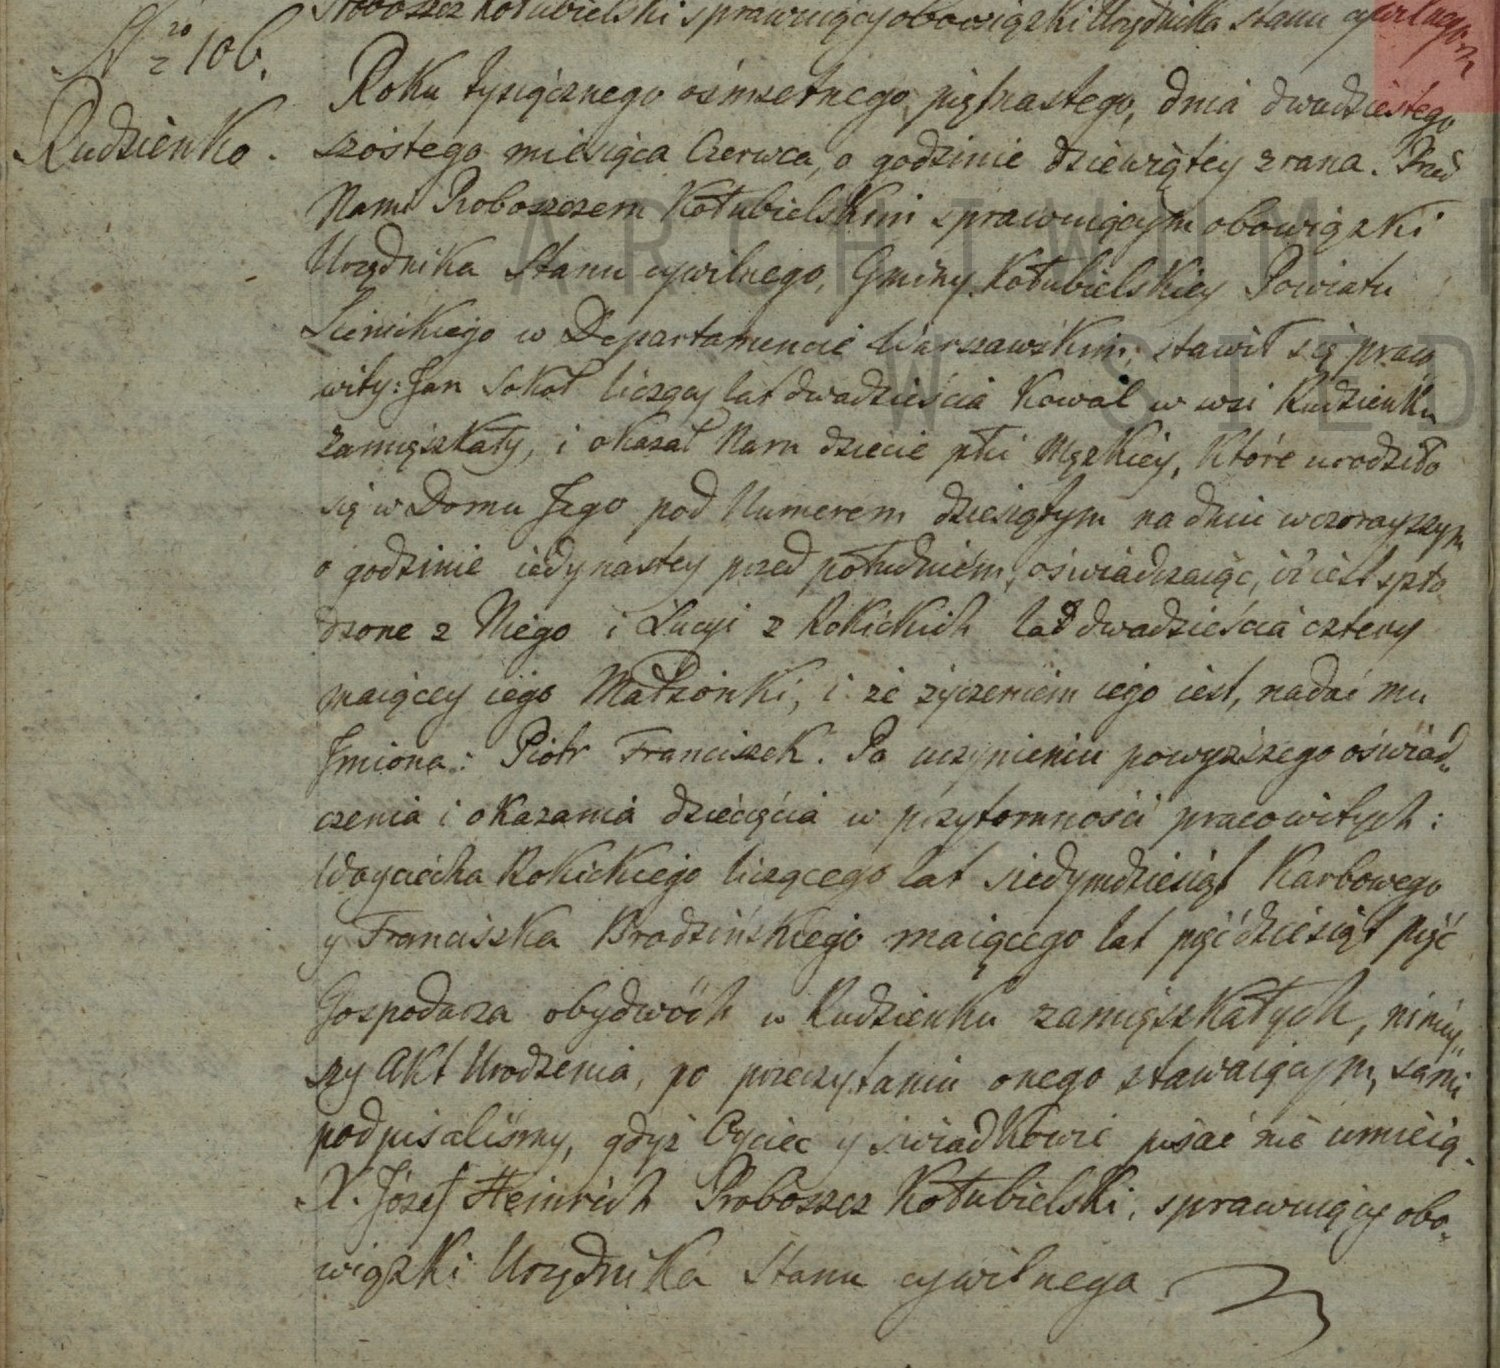
\includegraphics[width=1.0\linewidth]{
        1815_Piotr_Franciszek_Sokół_Gumulski_akt_chrztu_parafia_Kołbiel_wpis_106.jpg}
    \captionsetup{format=hang}
    \caption{Akt narodzin Piotra Franciszka Gomoły - par. Kołbiel 1815~rok 
    (106/1815) \cite{par_kolbiel1}.}
    \label{fig:pfgomola_1815}
\end{figure}

W~swoim akcie ślubu Anna Gomoła określana jest jako \enquote{Panna Anna, 
córka Antioniego i~Petronelli Gomułów gospodarzy niegdyś we wsi Mysłowie 
zamieszkałych, już nieżyjących, lat dwadzieścia sześć mającą, we wsi Mysłowie 
zrodzona, a~we wsi Rudnie w~służbie zamieszkała} W~akcie ślubu Krystyny 
Gomoły jest ona natomiast określana jako \enquote{Panna Krystyna, córka 
niegdyś Jędrzeja i~Agaty małżonków Gomulaków gospodarzy we wsi Wnętrznym 
zamieszkałych, lat dwadzieścia siedem mająca, we wsi Wnętrznym zrodzona, a~we 
wsi Rudzienku w~służbie zamieszkała}. Przytoczone powyżej opisy pasują w~stu 
procentach do, opisywanych w~poprzednim rozdziale niniejszej książki, Anny 
urodzonej w~1800~roku w~Mysłowie córki Antoniego i~Petronelli Gomołów oraz 
Krystyny urodzonej w~1798~roku we Wnętrznym córki Andrzeja i~Agaty Gomołów. 
Fakt, iż Anna i~Krystyna przybyły razem do Rudzienka, wzięły ślub tego samego 
dnia, a~jedna ożeniła się z~bratem stryjecznym drugiej, wzmacnia hipotezę 
o~bliskich, być może nawet braterskich, relacjach pomiędzy Antonim 
i~Andrzejem Gomołami.

\begin{figure}[!ht]
    \vspace*{0.5cm}
    \centering 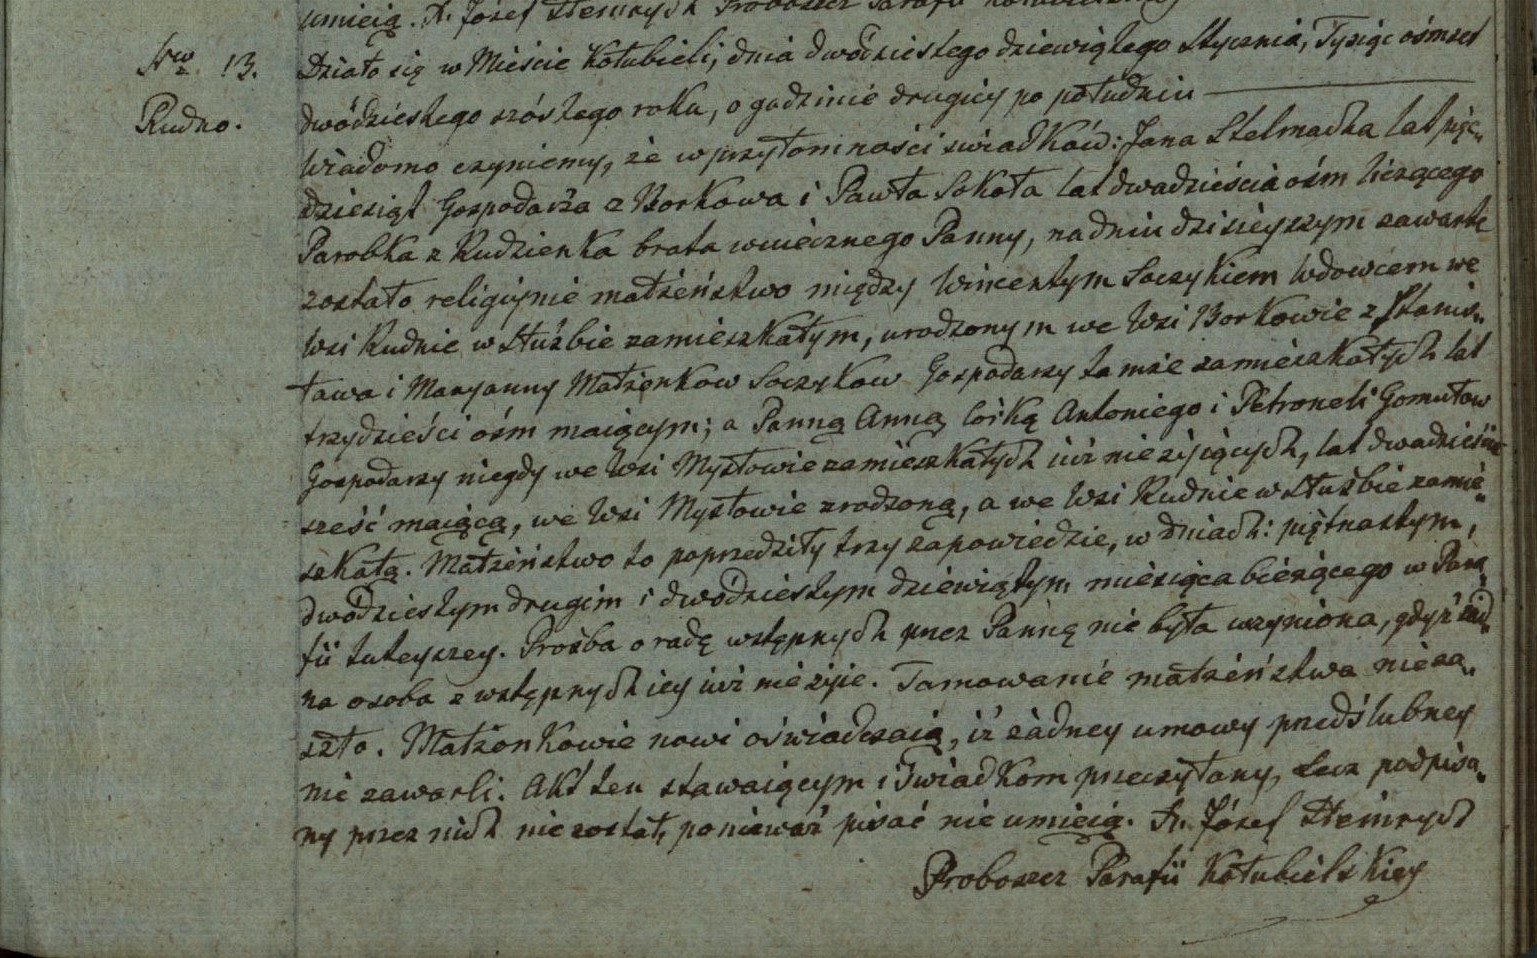
\includegraphics[width=0.92\linewidth]{
        1826_Anna_Gomoła_Wincenty_Soczyk_akt_ślubu_parafia_Kołbiel_wpis_13.jpg}
    \captionsetup{format=hang}
    \caption{Akt ślubu Anny Gomoły i~Wincenta Soczyka - par. Kołbiel 1826~rok 
    (13/1826) \cite{par_kolbiel1}.}
    \label{fig:agomola_1826}
\end{figure}

\begin{figure}[!ht]
    \vspace*{0.5cm}
    \centering 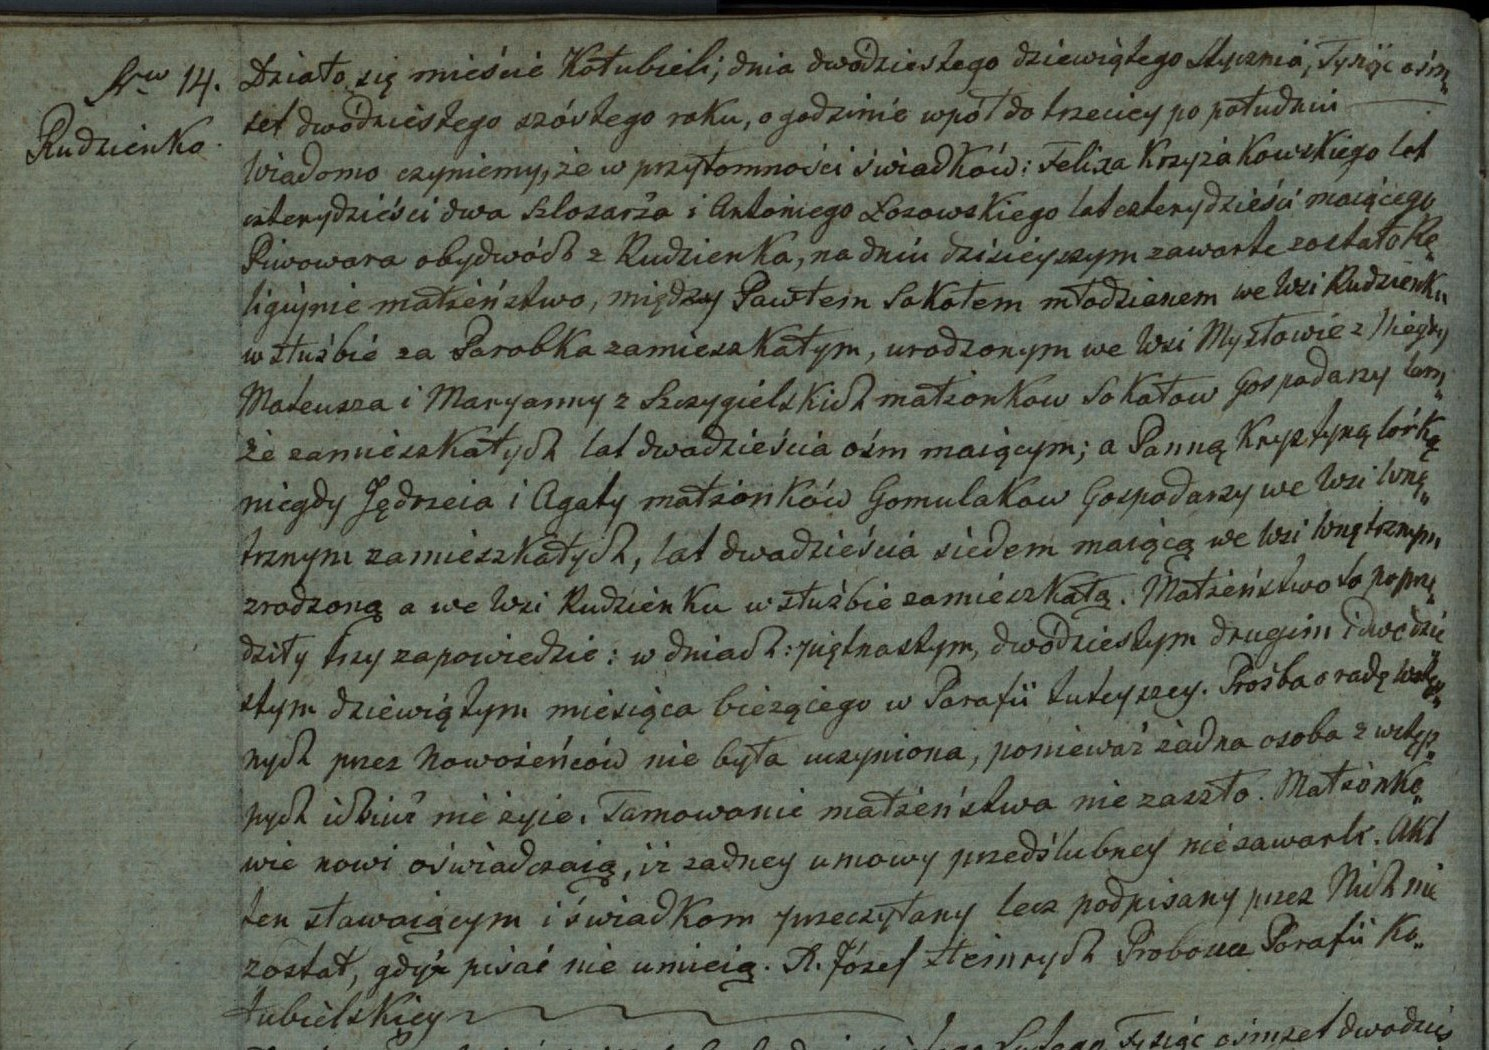
\includegraphics[width=0.92\linewidth]{
        1826_Krystyna_Gomoła_Paweł_Sokół_akt_ślubu_parafia_Kołbiel_wpis_14.jpg}
    \captionsetup{format=hang}
    \caption{Akt ślubu Krystyny Gomoły i~Pawła Sokoła - par. Kołbiel 1826~rok 
    (14/1826) \cite{par_kolbiel1}.}
    \label{fig:kgomola_1826}
\end{figure}

Anna Gomoła i~Wincenty Soczyk po ślubie zamieszkali w~pobliskiej wsi Borków, 
gdzie mieszkali do 1831~roku, kiedy to Wincenty zmarł. Para prawdopodobnie 
nie dochowała się potomstwa, a~przynajmniej nie ma informacji o~chrzcie ich 
dzieci w~obecnie dostępnych aktach metrykalnych parafii w~Kołbieli. 
W~1832~roku Anna wyszła ponownie za mąż, jej mężem został Jan Reszczyk 
(patrz: ryc. \ref{fig:agomola_1832}), po ślubie przeprowadzili się do jego 
rodzinnej wsi - do Lasomina pod Siennicą. Mieli wspólnie piątkę dzieci:

\begin{itemize}
    \item Damazego (ur. 1832~r. - ?),
    \item Juliannę (ur. 1834~r. - ?),
    \item Mariannę (ur. 1837~r. - ?),
    \item Stanisława (ur. 1838~r. - zm. 1843~r.),
    \item Józefę (ur. 1846~r. - zm. 1846~r.).
  \end{itemize}

  \begin{figure}[!ht]
    \vspace*{0.5cm}
    \centering 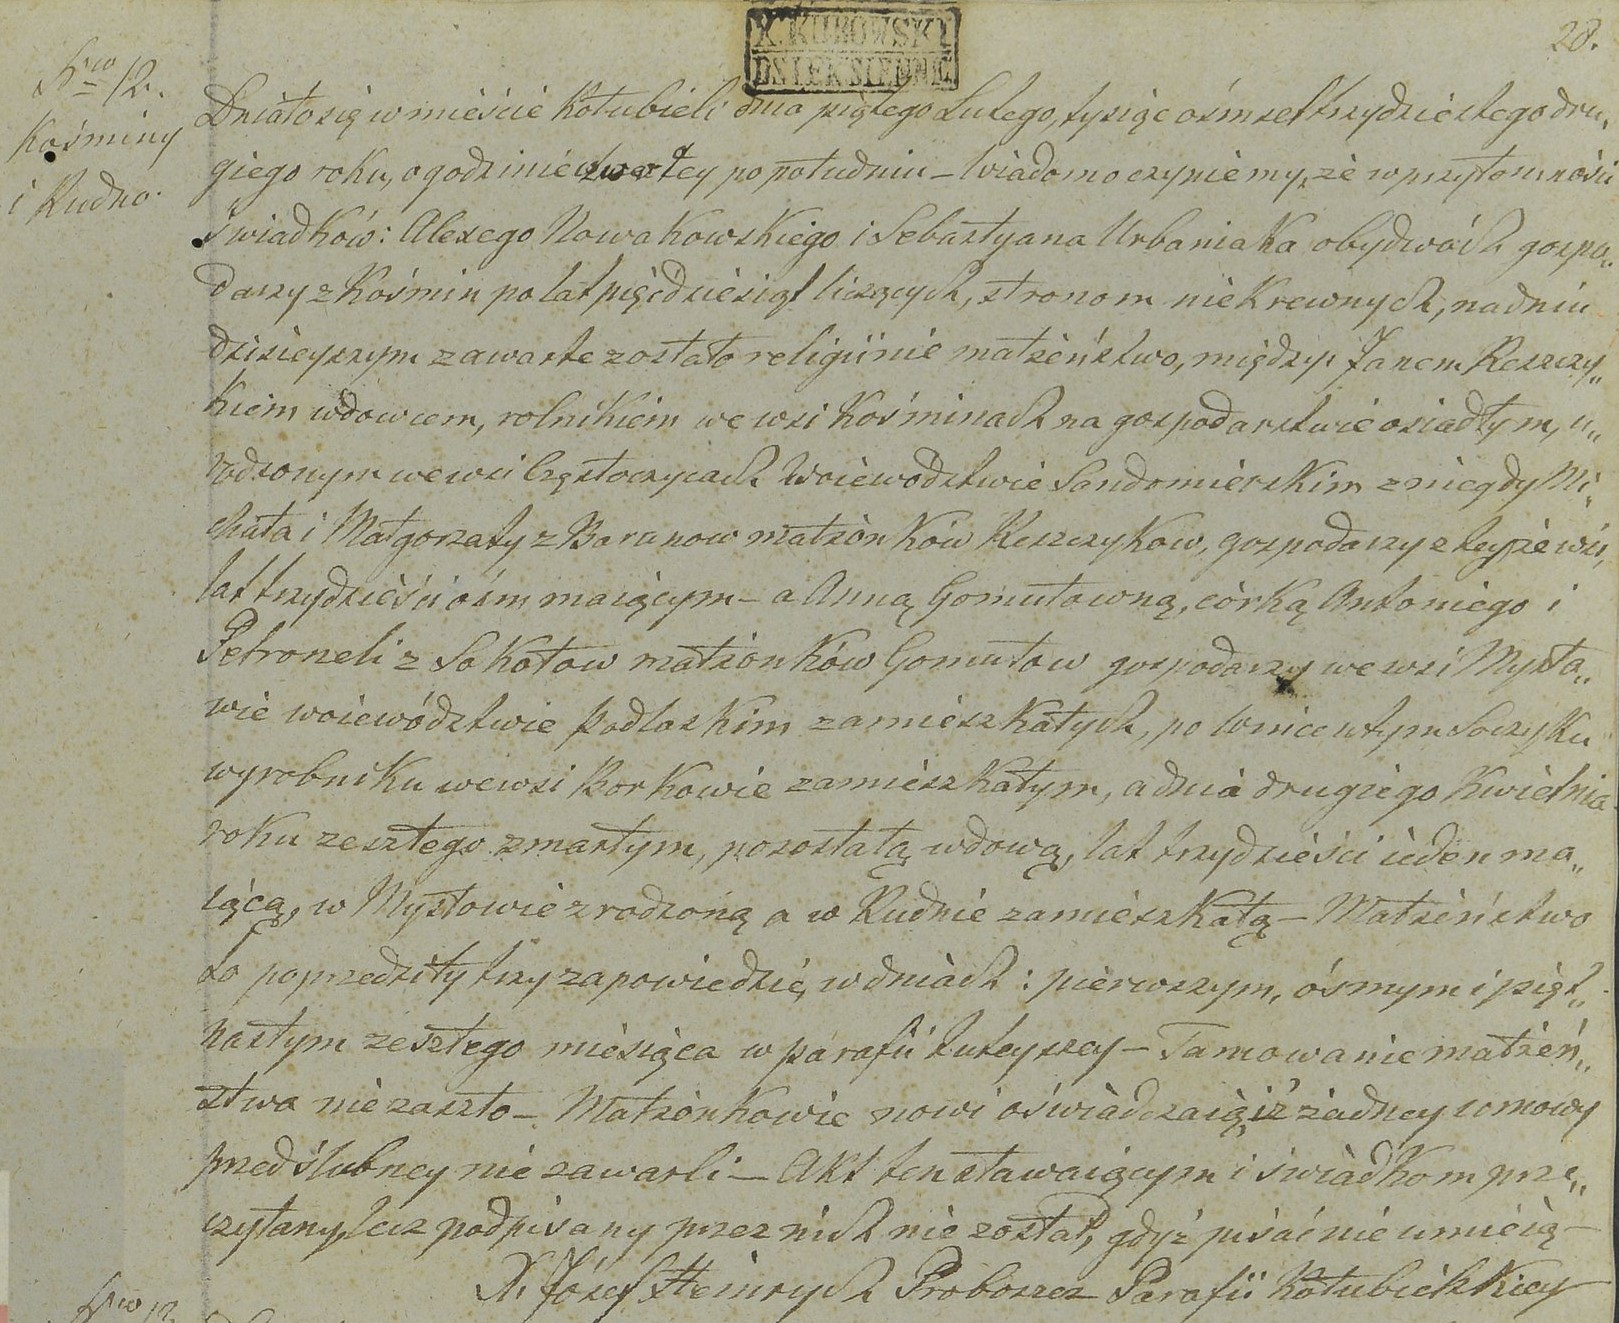
\includegraphics[width=1.0\linewidth]{
        1832_Anna_Gomoła_Jan_Reszczyk_akt_ślubu_parafia_Kołbiel_wpis_12.jpg}
    \captionsetup{format=hang}
    \caption{Akt ślubu Anny Soczyk (z~d.~Gomoła) i~Jana Reszczyka - par. 
    Kołbiel 1832~rok (12/1832) \cite{par_kolbiel1}.}
    \label{fig:agomola_1832}
\end{figure}

W~parafii pod wezwaniem św. Stanisława Biskupa i~Męczennika w~Siennicy nie 
sposób jest odnaleźć aktu zgonu Anny Reszczyk, pomimo, iż znajduje się tam 
akt zgonu jej męża Jana (z~1876~roku). Ostatnim wpisem w~księgach 
metrykalnych, w~którym wymieniona jest Anna, jest wpis z~1846~roku 
dokumentujący chrzest jej najmłodszej córki Józefy, gdzie została ona 
opisana w~następujący sposób: \enquote{...z~jego małżonki Anny z~Gumułów lat 
czterdzieści mającej...} (patrz: ryc. \ref{fig:jreszczyk_1846}).

\begin{figure}[!ht]
    \vspace*{0.5cm}
    \centering \includegraphics[width=1.0\linewidth]{
        1846_Józefa_Reszczyk_akt_chrztu_parafia_Siennica_wpis_8.jpg}
    \captionsetup{format=hang}
    \caption{Akt chrztu Józefy Reszczyk - par. Siennica 1846~rok (8/1846) 
    \cite{par_siennica}.}
    \label{fig:jreszczyk_1846}
\end{figure}

\begin{figure}[!ht]
    \vspace*{0.5cm}
    \centering 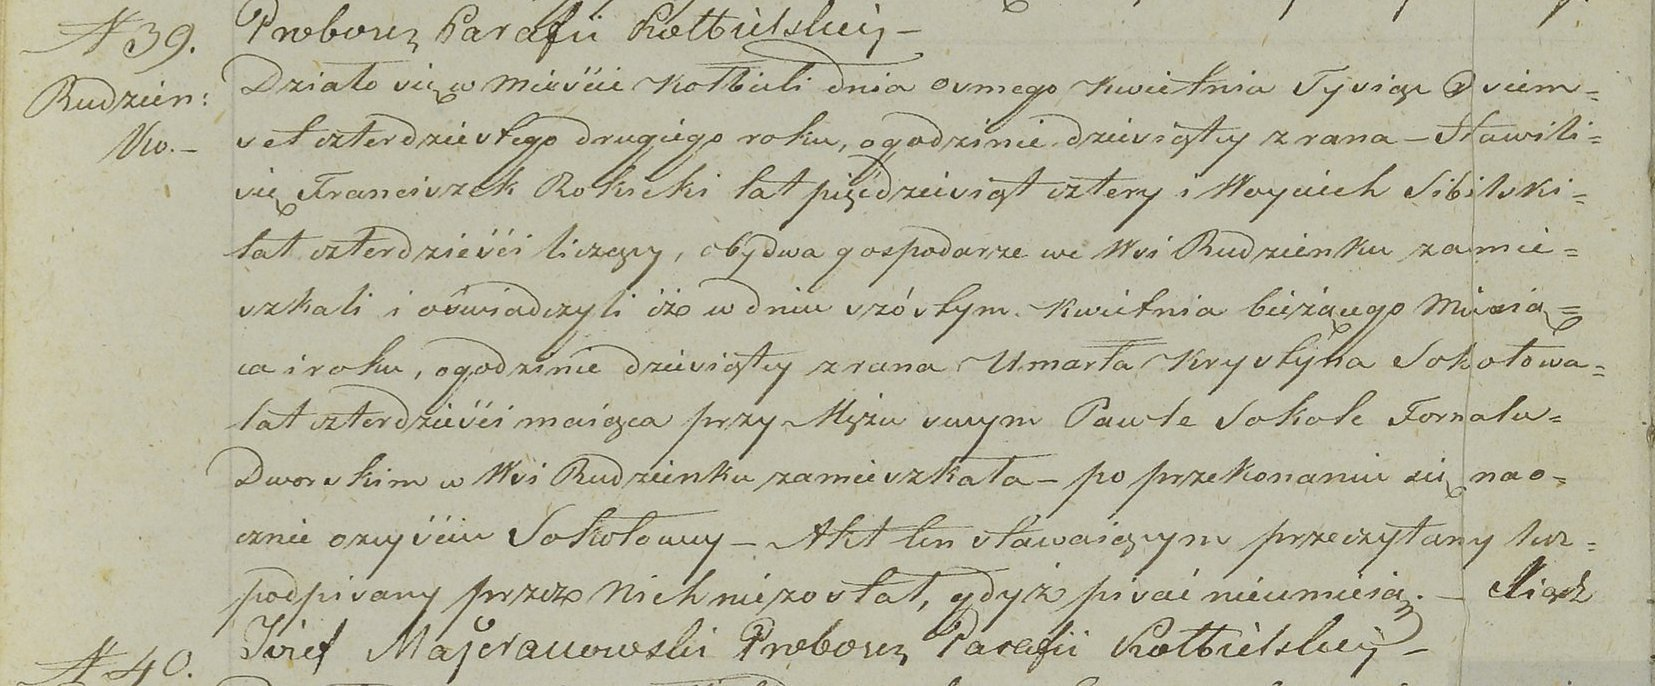
\includegraphics[width=1.0\linewidth]{
        1842_Krystyna_Gomoła_Sokół_akt_zgonu_parafia_Kołbiel_wpis_39.jpg}
    \captionsetup{format=hang}
    \caption{Akt zgonu Krystyny Sokół (z~d. Gomoły) - par. Kołbiel 1842~rok 
    (39/1842) \cite{par_kolbiel1}.}
    \label{fig:kgomola_1842}
\end{figure}

Krystyna i~Paweł Sokołowie resztę swojego życie spędzili w~Rudzienku, gdzie 
pracowali jako służący na tamtejszym dworze. Paweł był zatrudniony 
w~charakterze fornala dworskiego, czyli osoby zajmującej się końmi, nie 
wiadomo czym dokładnie na dworze Marianny z~Chrzanowskich zajmowała się jego 
żona Krystyna. Dochowali się siódemki potomstwa: 

\begin{itemize}
    \item Kunegundy (ur. 1825~r. - zm. 1828~r.),
    \item Marianny (ur. 1828~r. - zm. ?),
    \item Józefa (ur. 1832~r. - zm. ?),
    \item Jana I~(ur. 1834~r. - zm. ?),
    \item Jana II~(ur. 1836~r. - zm. ?),
    \item Teodora (ur. 1839~r. - zm. 1909~r.)\footnote{Co ciekawe syn 
    Teodora, Piotr Sokół, zmarł w~1930~roku w~Skrudzie, czyli we wsi 
    sasiadującej z~Desnem, w~którym mieszkali na początku XX~wieku 
    bezpośredni potomkowie Jana Gomoły.},
    \item Wojciecha (ur. 1842~r. - zm. 1842~r.).
  \end{itemize}

  \begin{figure}[!ht]
    \vspace*{0.5cm}
    \centering 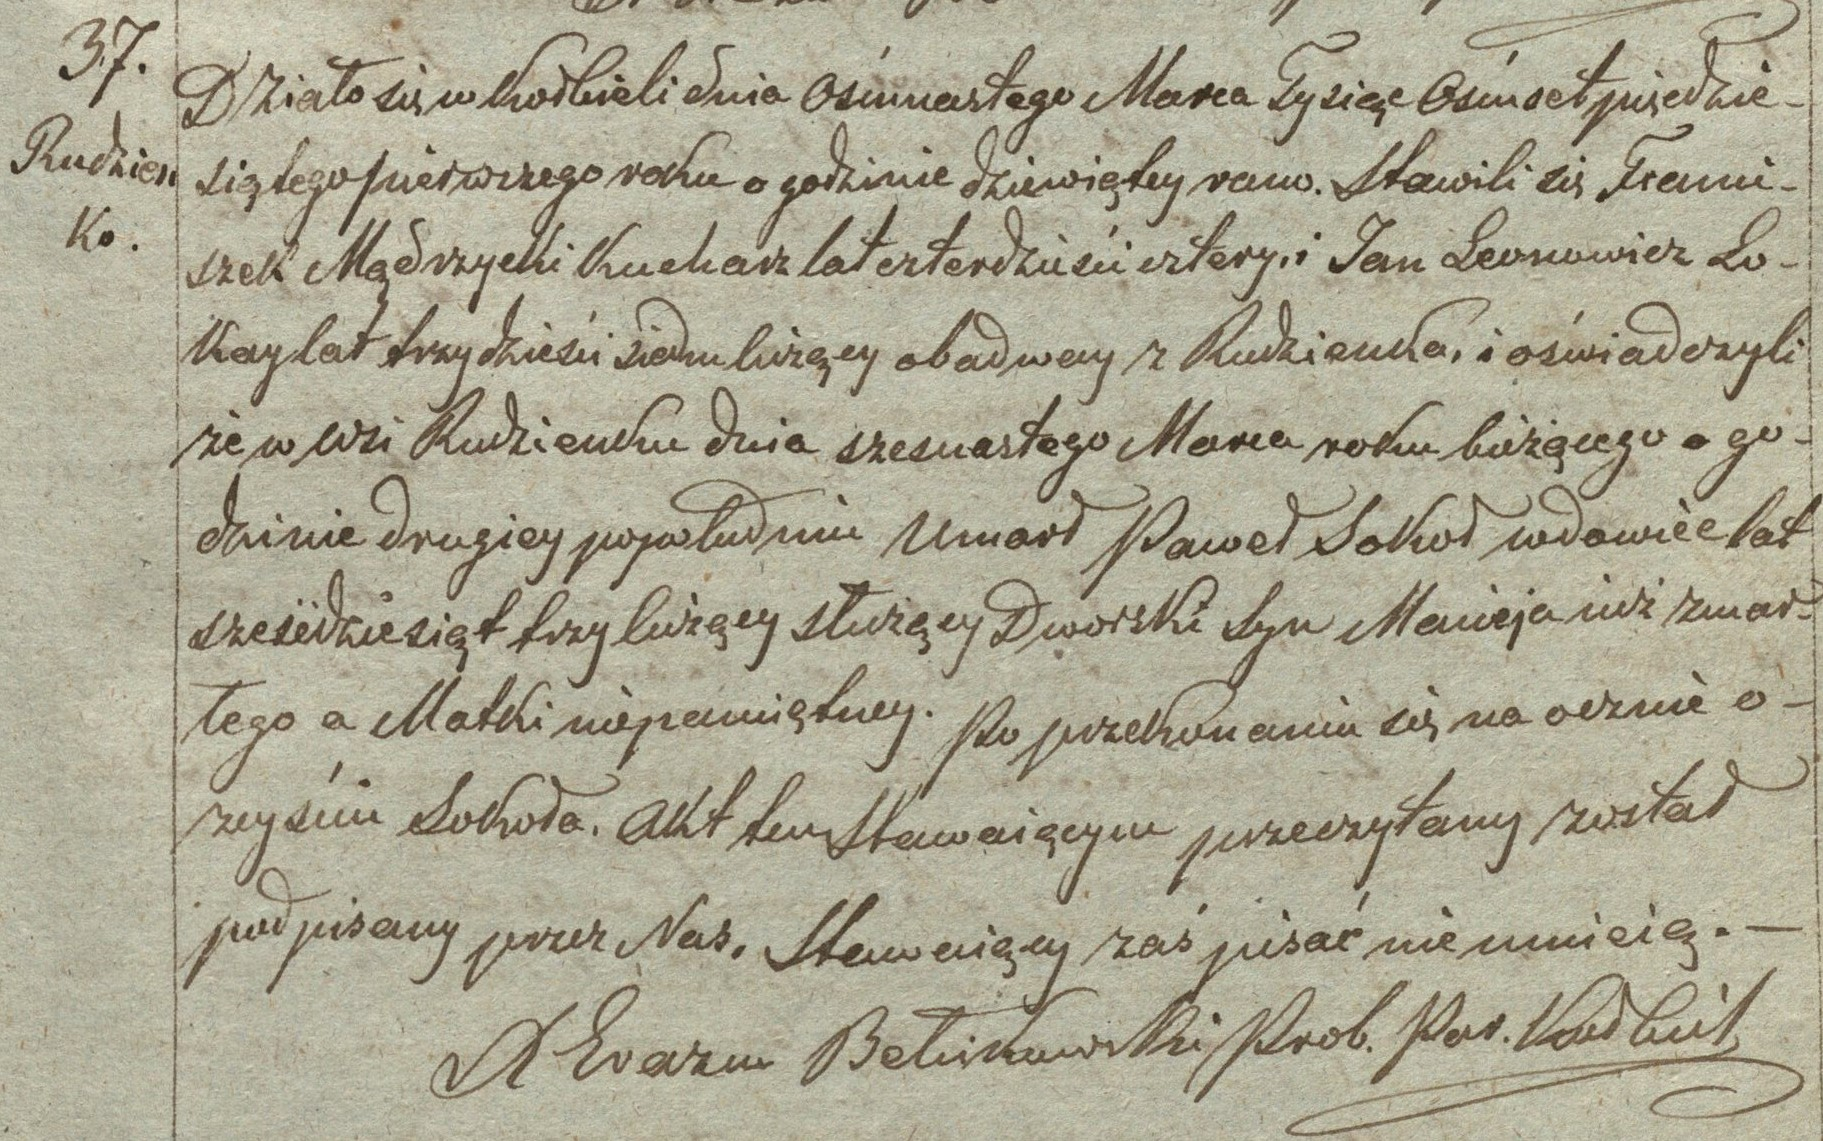
\includegraphics[width=1.0\linewidth]{
        1851_Paweł_Sokół_akt_zgonu_parafia_Kołbiel_wpis_37.jpg}
    \captionsetup{format=hang}
    \caption{Akt zgonu Pawła Sokoła - par. Kołbiel 1851~rok (37/1851) 
    \cite{par_kolbiel1}.}
    \label{fig:psokol_1851}
\end{figure}

Krystyna Sokół (z~domu Gomoła) zmarła 6~kwietnia 1842~roku, w~wieku 43~lat 
(patrz: ryc. \ref{fig:kgomola_1842}), a~jej mąż Paweł zmarł 16~marca 
1851~roku, w~wieku 53~lat (patrz: ryc. \ref{fig:psokol_1851}).

\clearpage
% Przednia okładka podrozdziału
\includepdf{Zamienie_mapa_fin2.png}

\section{Zamienie: 1820~r. - 1839~r.}

Wieś Zamienie na początku XIX~wieku znajdowała się na terenie zaboru 
austriackiego, następnie w~1809 roku została włączona do Księstwa 
Warszawskiego a~w~1815~roku do Królestwa Polskiego. Do momentu utraty przez 
Polskę niepodległości była częścią ziemi czerskiej województwa mazowieckiego. 
Najbliższymi dużymi ośrodkami miejskimi dla Zamienia były: oddalony o~około 
5~kilometrów na północny wschód Mińsk Mazowiecki oraz oddalona o~około 
10~kilometrów na południowy zachód Kołbiel. Zamienie należało w~tamtym czasie 
do parafii rzymskokatolickiej pod wezwaniem Narodzenia Najświętszej Maryi 
Panny w~Mińsku Mazowieckim. Najstarsza znana wzmianka o~Zamieniu pochodzi 
z~1476~roku ze zbioru dyplomatów\footnote{Dyplomat - w~średniowieczu dokument 
urzędowy poświadczający dokonanie danej czynności prawnej} księcia 
mazowieckiego Konrada III~Rudego, gdzie wspomina się o~Janie z~Zamienia (łac. 
\emph{Johannes de Zamyenye}) jako właścicielu wsi Zamienie, Niedziałka, Osiny 
i~Stojadła znajdujących się w~powiecie czerskim - patrz ryc. 
\ref{fig:zamienie_1476}. Na początku XIX~wieku Zamienie było częścią dóbr 
Rudzienko należących do chorążego warszawskiego Marcina Chrzanowskiego 
z~Chrzanowa Wielkiego i~Małego (herbu Korab), po 1811~roku dobra te 
odziedziczyła jego córka Marianna z~Chrzanowskich, która była ich 
właścicielką aż do śmierci w~1860~roku.

\begin{figure}[!ht]
    \vspace*{0.5cm}
    \centering 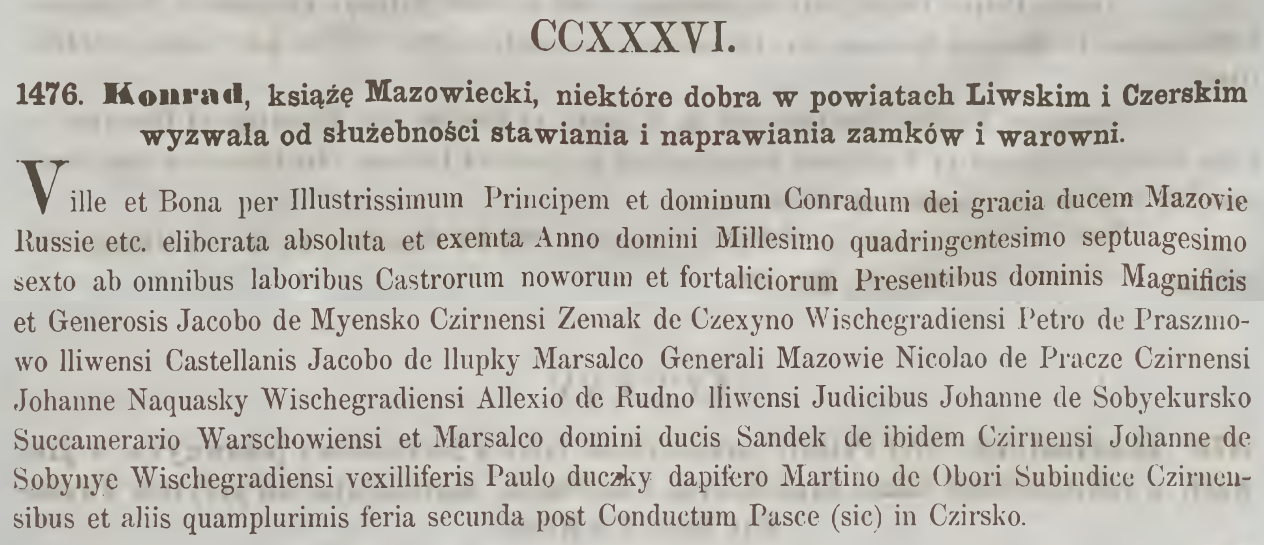
\includegraphics[width=1.0\linewidth]{Zamienie_1476.png}

    \vspace*{0.5cm}

    \centering 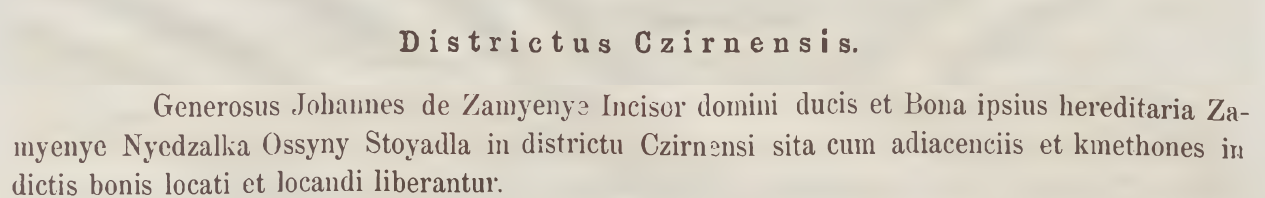
\includegraphics[width=1.0\linewidth]{Zamienie_1476_2.png}
    \captionsetup{format=hang}
    \caption{Wpis dotyczący Jana z~Zamienia pochodzący ze zbioru dyplomatów 
    księcia mazowieckiego Konrada III~Rudego z~1476~roku \cite{jlubomirski2}.}
    \label{fig:zamienie_1476}
\end{figure}

Jan Gomoła wraz ze swoją żoną Łucją oraz synem Piotrem Franciszkiem 
przeprowadzili się do Zamienia prawdopodobnie około 1820~roku. Świadczą o~tym 
skany ksiąg parafialnych parafii w~Mińsku Mazowieckim dostępne na portalu 
\emph{szukajwarchiwach.gov.pl}\footnote{Akta metrykalne parafii pod wezwaniem 
Narodzenia Najświętszej Maryi Panny w~Mińsku Mazowieckim z~lat 1810-1921 
dostępne są pod adresami: \\
\url{https://www.szukajwarchiwach.gov.pl/en/zespol/-/zespol/56785} (dostęp: 
marzec 2024 r.) \\ 
\url{https://www.szukajwarchiwach.gov.pl/en/zespol/-/zespol/56408}(dostęp: 
marzec 2024 r.).}. Dnia 1~lipca 1820~roku urodził się drugi syn Jana i~Łucji 
Gomołów - Franciszek. Jak wynika z~aktu jego narodzin, urodził się on 
w~Zamieniu, w~domu swojego ojca Jana, pod numerem dwudziestym drugim. Jan 
Gomoła w~akcie narodzin Franciszka został nazwany Janem Gumulskim: 
\enquote{...pracowity Jan Gumulski kowal z~Zamienia lat trzydzieści...}.

\begin{figure}[!ht]
    \vspace*{0.5cm}
    \centering \includegraphics[width=1.0\linewidth]{
        1820_Franciszek_Gumulski_akt_chrztu_parafia_Mińsk_Mazowiecki_wpis_144.jpg}
    \captionsetup{format=hang}
    \caption{Akt narodzin Franciszka I Gumulskiego - par. Mińsk Mazowiecki 
    1820~rok (144/1820) \cite{par_minsk1}.}
    \label{fig:fgumulski_1820}
\end{figure}

Dnia 9~grudnia 1823~roku urodził się trzeci syn Jana i~Łucji Gomołów. Syn ten 
podobnie jak dwaj poprzedni nosił imię Franciszek. Zwyczaj nadawania tych 
samych imion kolejnym swoim dzieciom był praktykowany w~XIX wieku na ziemiach 
polskich, ale zazwyczaj powtórzone imiona nadawano noworodkom, gdy starsze 
dziecko przedwcześnie zmarło. W~tym przypadku Jan i~Łucja Gomołowie 
zdecydowali się nadać imię Franciszek swojemu trzeciemu synowi, gdy jego dwaj 
starsi bracia jeszcze żyli, co było rzadko spotykaną w~tamtych czasach 
praktyką. W~akcie narodzin swojego trzeciego syna Jan Gomoła ponownie został 
określony jako \enquote{Jan Gumulski kowal z~Zamienia} (patrz: ryc. 
\ref{fig:fgumulski_1823}).

\begin{figure}[!ht]
    \vspace*{0.5cm}
    \centering \includegraphics[width=1.0\linewidth]{
        1823_Franciszek_Gumulski_akt_chrztu_parafia_Mińsk_Mazowiecki_wpis_270.jpg}
    \captionsetup{format=hang}
    \caption{Akt narodzin Franciszka II Gumulskiego - par. Mińsk Mazowiecki 
    1823~rok (270/1823) \cite{par_minsk1}.}
    \label{fig:fgumulski_1823}
\end{figure}

Czwarty syn Jana i~Łucji przyszedł na świat niemal równo sześć lat po 
narodzinach ich trzeciego syna. Dnia 4 grudnia 1829~roku w~Zamieniu urodził 
się Andrzej Gumulski, w~akcie chrztu przedstawiono go jako syna Jana, kowala 
z~Zamienia, oraz Łucji z~Rokickich (patrz: ryc. \ref{fig:agumulski_1829}). 
W~latach 1810-1826, na ziemiach polskich, akta chrztu, spisywane wcześniej po 
łacinie przez księży katolickich, zostały zastąpione przez akta narodzin, 
które spisywali również księża, ale już w~języku polskim oraz działając 
w~charakterze urzędników stanu cywilnego. Od 1827~roku wrócono ponownie do 
rejestracji akt chrztu, zaczęto je jednak spisywać po polsku (w~odróżnieniu 
do czasów sprzed 1810~roku), stąd też w~przypadku Andrzeja Gumulskiego 
(w~przeciwieństwie do jego pozostałych braci, dla których dysponujemy tylko 
aktami narodzin) możemy dokładnie wskazać, iż jego rodzicami chrzestnymi 
zostali Mateusz Zielechowski oraz Agnieszka Rokicka (z~domu Rudnicka) żona 
Jana Rokickiego brata stryjecznego Łucji Gomoły.

\begin{figure}[!ht]
    \vspace*{0.5cm}
    \centering \includegraphics[width=1.0\linewidth]{
        1829_Andrzej_Gumulski_akt_chrztu_parafia_Mińsk_Mazowiecki_wpis_258.jpg}
    \captionsetup{format=hang}
    \caption{Akt chrztu Andrzeja Gumulskiego - par. Mińsk Mazowiecki 
    1829~rok (258/1829) \cite{par_minsk2}.}
    \label{fig:agumulski_1829}
\end{figure}

\begin{figure}[!ht]
    \vspace*{0.5cm}
    \centering \includegraphics[width=1.0\linewidth]{
        1830_Franciszek_Gumulski_akt_zgonu_parafia_Mińsk_Mazowiecki_wpis_180.jpg}
    \captionsetup{format=hang}
    \caption{Akt zgonu Franciszka II Gumulskiego - par. Mińsk Mazowiecki 
    1830~rok (180/1830) \cite{par_minsk2}.}
    \label{fig:fgumulski_1830_1}
\end{figure}

Rok po narodzinach Andrzeja Gumulskiego, w~grudniu 1830~roku, umiera dwóch 
z~trzech jego starszych braci: Franciszek II~Gumulski oraz 
Franciszek I~Gumulski. Najpierw czwartego grudnia 1830~roku umiera młodszy 
z~braci, siedmiolatek urodzony w~1823~roku (patrz: 
ryc. \ref{fig:fgumulski_1830_1}), a~następnie 26~grudnia 1830~roku umiera 
jego trzy lata starszy brat, dziesięciolatek urodzony w~1820~roku (patrz: ryc. 
\ref{fig:fgumulski_1830_2}). \textbf{Akt zgonu siedmioletniego Franciszka 
II~Gumulskiego jest pierwszym historycznie dokumentem, w~drzewie 
genealogicznym rodziny Gomulskich z~Desna, w~którym pojawia się nazwisko 
\enquote{Gomulski}} i~to co najmniej dwukrotnie - nowe nazwisko rodziny 
Jana Gomoły pada w~akcie zgonu Franciszka II~czterokrotnie, dwa pierwsze 
zapisy wskazują raczej na nazwisko \enquote{Gomolski} niż \enquote{Gomulski}, 
co do dwóch ostatnich zapisów nie ma już takich wątpliwości - jasno wynika 
z~nich, iż chodzi o~osoby o~nazwisku \enquote{Gomulski}.

\begin{figure}[!ht]
    \vspace*{0.5cm}
    \centering \includegraphics[width=1.0\linewidth]{
        1830_Franciszek_Gumulski_akt_zgonu_parafia_Mińsk_Mazowiecki_wpis_208.jpg}
    \captionsetup{format=hang}
    \caption{Akt zgonu Franciszka I Gumulskiego - par. Mińsk Mazowiecki 
    1830~rok (208/1830) \cite{par_minsk2}.}
    \label{fig:fgumulski_1830_2}
\end{figure}

Najmłodszym dzieckiem, które urodziło się ze związku Jana i~Łucji Gomołów, 
była Marianna. Urodziła się ona dnia 27~listopada 1832~roku w~Zamieniu, a~jej 
rodzicami chrzestnymi zostali Michał Rutkowski oraz Marianna Rokicka (z~domu 
Stelmach) żona Franciszka Rokickiego kuzyna Łucji Gomoły. \textbf{Marianna 
Gomulska była pierwszą osobą z~drzewa genealogicznego rodziny Gomulskich 
z~Desna, która w~świetle dokumentów kościelnych, nosiła nazwisko 
\enquote{Gomulski}} - w~akcie jej chrztu, jej ojciec Jan Gomoła, został 
określony jako \enquote{...Jan Gomulski kowal w~Zamieniu zamieszkały lat 
czterdzieści mający...} (patrz: ryc. \ref{fig:mgomulska_1832_1}). Marianna 
Gomulska żyła bardzo krótko, zaledwie szesnaście dni, zmarła 12~grudnia 
1832~roku - w~akcie jej zgonu ponownie, dwukrotnie, pojawia się nazwisko 
\enquote{Gomulski} (patrz: ryc. \ref{fig:mgomulska_1832_2}).

\begin{figure}[!ht]
    \vspace*{0.5cm}
    \centering \includegraphics[width=1.0\linewidth]{
        1832_Marianna_Gomulska_akt_chrztu_parafia_Mińsk_Mazowiecki_wpis_231.jpg}
    \captionsetup{format=hang}
    \caption{Akt chrztu Marianny Gomulskiej - par. Mińsk Mazowiecki 1832~rok 
    (231/1832) \cite{par_minsk2}.}
    \label{fig:mgomulska_1832_1}
\end{figure}

\begin{figure}[!ht]
    \vspace*{0.5cm}
    \centering \includegraphics[width=1.0\linewidth]{
        1832_Marianna_Gomulska_akt_zgonu_parafia_Mińsk_Mazowiecki_wpis_233.jpg}
    \captionsetup{format=hang}
    \caption{Akt zgonu Marianny Gomulskiej - par. Mińsk Mazowiecki 1832~rok 
    (233/1832) \cite{par_minsk2}.}
    \label{fig:mgomulska_1832_2}
\end{figure}

Dnia 15 lutego 1835~roku, w~wieku niespełna dwudziestu lat, w~parafii pod 
wezwaniem Narodzenia Najświętszej Maryi Panny w~Mińsku Mazowieckim, Piotr 
Franciszek Gomoła z~Zamienia, wziął ślub z~szesnastoletnią Marianną Chłopik 
(patrz: ryc. \ref{fig:pfgumulski_1835}). Marianna przyszła na świat 
pierwszego stycznia 1819~roku w~Zamieniu jako córka Dominika Chłopika (ur. 
1786~r. - zm. 1858~r.) oraz Rozalii Chłopik (ur. 1786~r. - zm. 1862~r.), 
z~domu Zgutka (patrz: ryc. \ref{fig:mchlopik_1819}). 

\begin{figure}[!ht]
    \vspace*{0.5cm}
    \centering 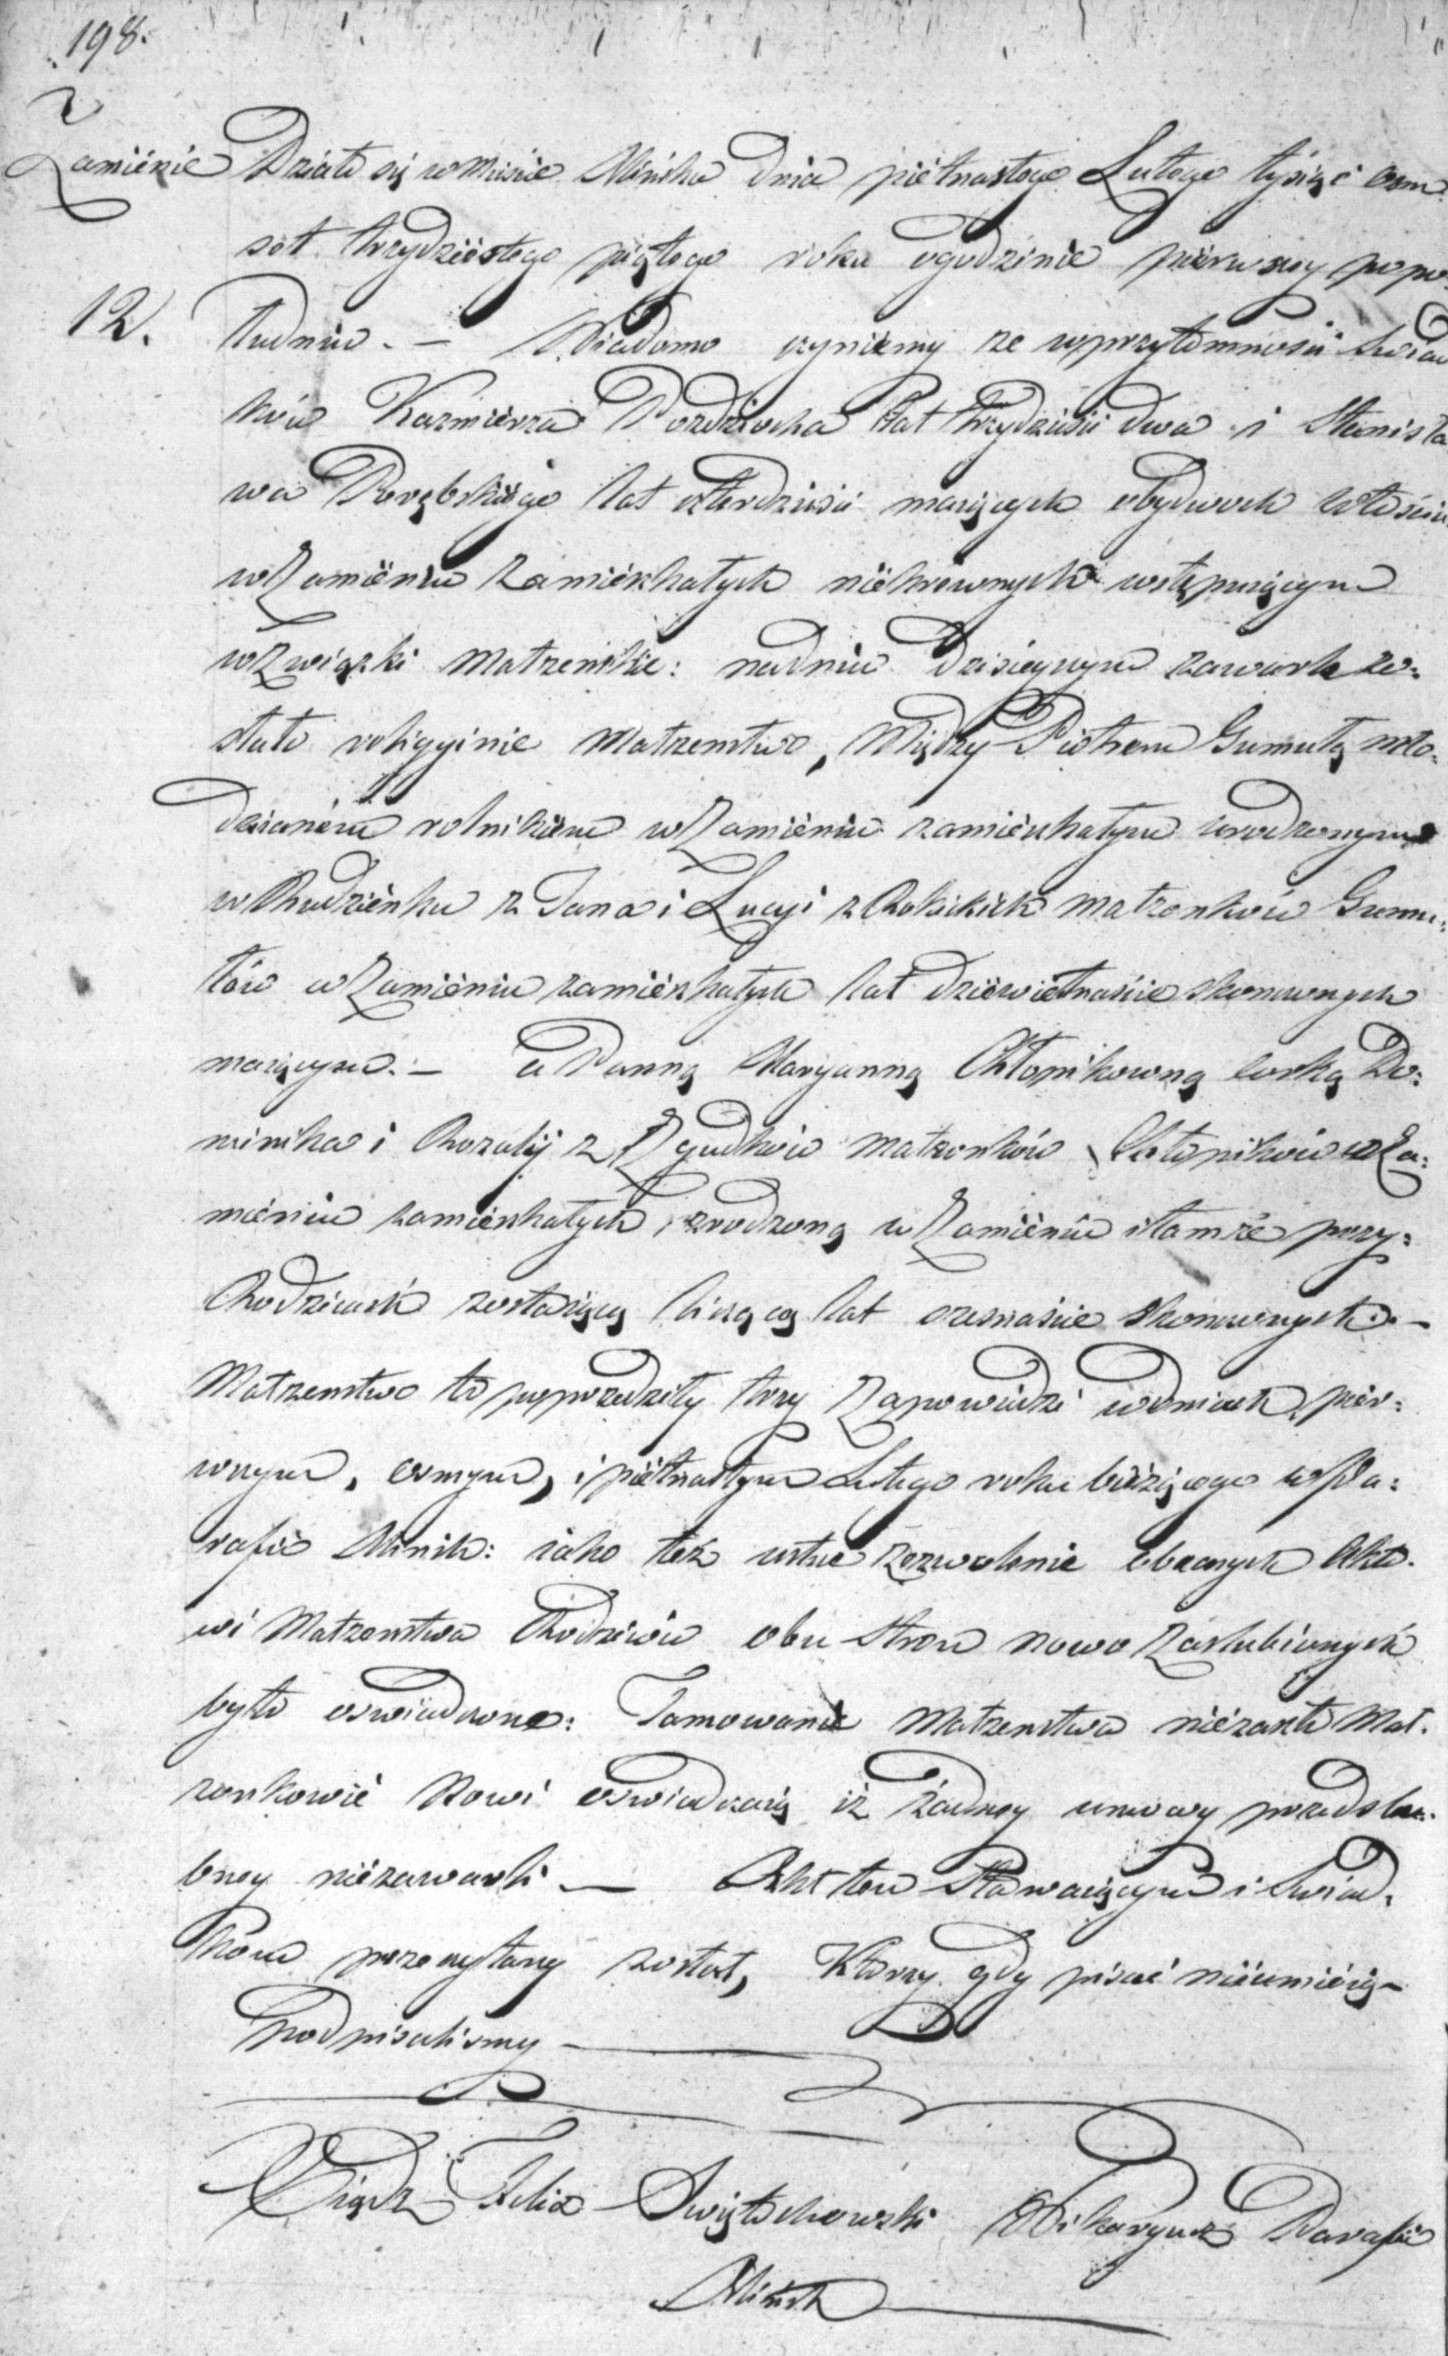
\includegraphics[width=0.85\linewidth]{
        1835_Piotr_Franciszek_Gumulski_Marianna_Chłopik_akt_ślubu_parafia_Mińsk_Mazowiecki_wpis_12.jpg}
    \captionsetup{format=hang}
    \caption{Akt ślubu Piotra Franciszka Gomoły oraz Marianny Chłopik - 
    par. Mińsk Mazowiecki 1835~rok (12/1835) \cite{par_minsk2}.}
    \label{fig:pfgumulski_1835}
\end{figure}

Rodzina Chłopików, podobnie jak rodzina Zgutków, wywodziła się ze stanu 
chłopskiego. Obie rodziny zamieszkiwały Zamienie co najmniej od połowy 
XVII~wieku. Dominik i~Rozalia Chłopikowie dochowali się trójki dzieci:

\begin{itemize}
    \item Franciszka (ur. 1814~r. - zm. ?),
    \item Marianny (ur. 1819~r. - zm. 1880~r.),
    \item Wojciecha (ur. 1823~r. - zm. 1896~r.).
\end{itemize}

Dominik Chłopik zmarł 3~kwietnia 1858~roku w~Zamieniu, dożywając wieku 
72~lat. Jego żona Rozalia żyła 4~lata dłużej - zmarła 7~czerwca 1862~roku 
w~swojej rodzinnej wsi.

\begin{figure}[!ht]
    \vspace*{0.5cm}
    \centering 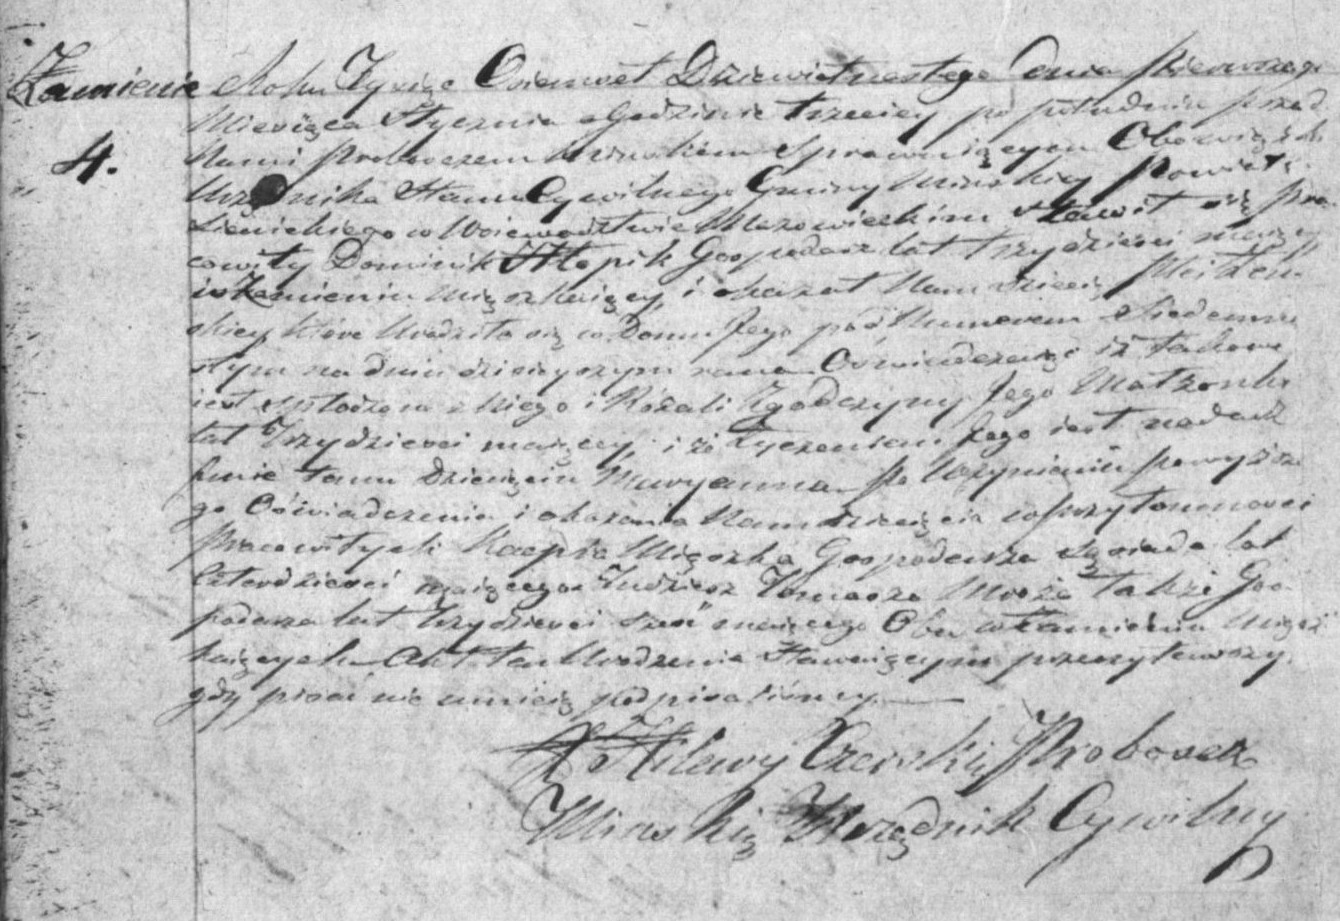
\includegraphics[width=1.0\linewidth]{
        1819_Marianna_Gumulska_Chłopik_akt_chrztu_parafia_Mińsk_Mazowiecki_wpis_4.jpg}
    \captionsetup{format=hang}
    \caption{Akt narodzin Marianny Chłopik - par. Mińsk Mazowiecki 1819~rok 
    (4/1819) \cite{par_minsk1}.}
    \label{fig:mchlopik_1819}
\end{figure}

Piotr Franciszek Gumulski wraz z~żoną Marianną przez pierwsze kilka lat po 
swoim ślubie mieszkali w~Zamieniu. Tam też 29 maja 1836~roku urodził się ich 
pierwszy syn Jan Gomulski\footnote{W~akcie jego chrztu wskazane jest 
wprawdzie nazwisko Gumulski, ale wszystkich członków rodziny Gomulskich 
z~Desna, począwszy od czwartego pokolenia, będziemy w~niniejszej książce, dla 
porządku, nazywać Gomulskimi.} (patrz: ryc. \ref{fig:jgomulski_1836}). 
Rodzicami chrzestnymi Jana zostali Jan Zgutka oraz Anna Ładno, a~w~akcie jego 
chrztu, jego ojciec Piotr Franciszek, został określony jako \enquote{...Piotr 
Gumulski parobek lat trzydzieści z~Zamienia...}.

\begin{figure}[!ht]
    \vspace*{0.5cm}
    \centering \includegraphics[width=1.0\linewidth]{
        1836_Jan_Gumulski_akt_chrztu_parafia_Mińsk_Mazowiecki_wpis_120.jpg}
    \captionsetup{format=hang}
    \caption{Akt chrztu Jana Gomulskiego - par. Mińsk Mazowiecki 1836~rok 
    (120/1836) \cite{par_minsk2}.}
    \label{fig:jgomulski_1836}
\end{figure}

Około 1839~roku Piotr Franciszek Gumulski wraz z~żoną Marianną oraz 
trzyletnim synem Janem przeprowadzili się do oddalonej o~sześć kilometrów na 
południowy wschód wsi Grzebowilk. Wszystko wskazuje na to, iż przy tej 
przeprowadzce towarzyszyli im również rodzice Piotra Jan i~Łucja Gomołowie 
oraz jego dziesięcioletni brat Andrzej.

\clearpage
% Przednia okładka podrozdziału
\includepdf{Grzebowilk_mapa_fin.png}

\section{Grzebowilk: 1839~r. - 1853~r.}

Wieś Grzebowilk na początku XIX~wieku znajdowała się na terenie zaboru 
austriackiego, następnie w~1809~roku została włączona do Księstwa 
Warszawskiego a~w~1815~roku do Królestwa Polskiego. Do momentu utraty przez 
Polskę niepodległości była częścią ziemi czerskiej województwa mazowieckiego. 
Najbliższymi dużymi ośrodkami miejskimi dla Grzebowilka były: oddalona 
o~około siedem kilometrów na południowy zachód Kołbiel oraz oddalony o~około 
siedem kilometrów na północny wschód Mińsk Mazowiecki. Grzebowilk należał 
w~tamtym czasie do parafii pod wezwaniem Świętej Trójcy w~Kołbieli. 
Najstarsza znana wzmianka o~Grzebowilku pochodzi z~1564~roku - wieś ta 
została opisana w~lustracjach starostwa osieckiego z~lat 1564-1569 
\cite{agad2} (patrz: ryc. \ref{fig:jgomulski_1836}). W~XV~wieku wieś 
Grzebowilk była własnością sędziego liwskiego i~chorążego zakroczymskiego 
Aleksego z~Gościańczyc, a~potem do końca XVIII~wieku do potomków tego rodu. 
Na przełomie XVIII~i~XIX wieku w~Grzebowilku wzniesiono drewniany dwór 
myśliwski, który w~XIX~wieku został wymieniony wśród nadań księcia Józefa 
Poniatowskiego \cite{klos}.

\begin{figure}[!ht]
    \vspace*{0.5cm}
    \centering 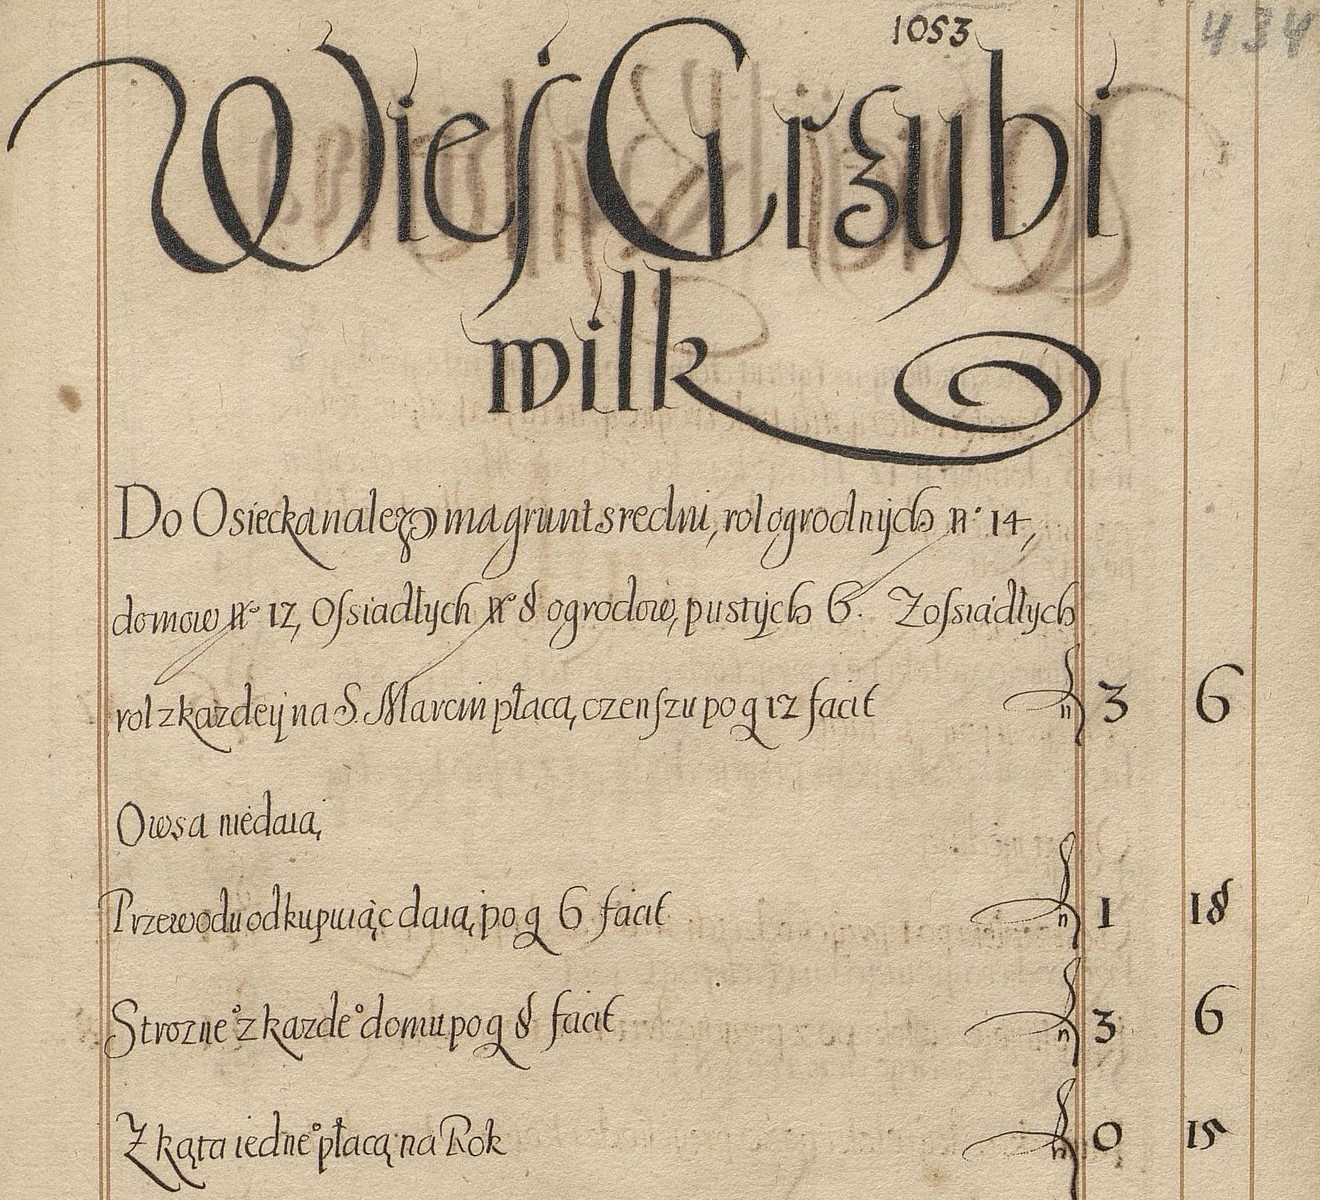
\includegraphics[width=0.9\linewidth]{
        Grzebowilk_1564.jpg}
    \captionsetup{format=hang}
    \caption{Pierwszy znany wpis dotyczący wsi Grzebowilk pochodzący 
    z~1564~roku z~lustracji starostwa osieckiego \cite{agad2}.}
    \label{fig:grzebowilk_1564}
\end{figure}

\begin{figure}[!ht]
    \vspace*{0.5cm}
    \centering \includegraphics[width=0.95\linewidth]{
        1839_Karolina_Gumulska_akt_chrztu_parafia_Kołbiel_wpis_100.jpg}
    \captionsetup{format=hang}
    \caption{Akt chrztu Karoliny Gomulskiej - par. Kołbiel 1839~rok (100/1839) 
    \cite{par_kolbiel2}.}
    \label{fig:kgomulska_1839}
\end{figure}

\begin{figure}[!ht]
    \vspace*{0.5cm}
    \centering \includegraphics[width=0.95\linewidth]{
        1840_Karolina_Gumulska_akt_zgonu_parafia_Kołbiel_wpis_4.jpg}
    \captionsetup{format=hang}
    \caption{Akt zgonu Karoliny Gomulskiej - par. Kołbiel 1840~rok (4/1840) 
    \cite{par_kolbiel2}.}
    \label{fig:kgomulska_1840}
\end{figure}

Pierwszym dzieckiem Piotra i~Marianny Gumulskich, które urodziło się 
w~Grzebowilku, była Karolina Gomulska. Urodziła się ona 26~~października 
1839~roku, a~jej rodzicami chrzestnymi zostali Franciszek Chłopik, starszy 
brat jej matki, oraz Ludwika Bojemska (patrz: ryc. \ref{fig:kgomulska_1839}). 
Ojciec Karoliny Gomulskiej w~akcie jej chrztu został określony jako 
\enquote{...Piotr Gumulski owczarz we wsi Grzebowilku zamieszkały lat 
dwadzieścia trzy mający...} - wpis ten jest o~tyle ciekawy, że w~żadnym 
innym późniejszym dokumencie Piotr Gumulski nie został określony jako 
\enquote{owczarz}, zawód ten w~XIX~wieku był zawodem bardzo prestiżowym na 
ziemiach polskich, przekazywanym często z~ojca na syna, a~w~rodzinie 
Gomołów / Gomulskich nie sposób jest odnaleźć takich tradycji. Karolina 
Gomulska żyła niewiele ponad 2,5 miesiąca - zmarła dziewiątego stycznia 
1840~roku (patrz: ryc. \ref{fig:kgomulska_1840}).

\begin{figure}[!ht]
    \vspace*{0.5cm}
    \centering \includegraphics[width=1.0\linewidth]{
        1840_Grzegorz_Gomulski_akt_chrztu_parafia_Kołbiel_wpis_152.jpg}
    \captionsetup{format=hang}
    \caption{Akt chrztu Grzegorza Gomulskiego - par. Kołbiel 1840~rok 
    (152/1840) \cite{par_kolbiel2}.}
    \label{fig:ggomulski_1840}
\end{figure}

Dnia 26 listopada 1840~roku na świat przyszedł drugi syn Piotra i~Marianny 
Gumulskich - Grzegorz Gomulski. Jego rodzicami chrzestnymi zostali Mateusz 
Bojemski oraz Krystyna Nowak (patrz: ryc. \ref{fig:ggomulski_1840}). Ojciec 
Grzegorza w~akcie jego chrztu został określony jako \enquote{...Piotr 
Gomulski lat dwadzieścia sześć mający gospodarz z~Grzebowilka...}. Trzecim 
dzieckiem małżonków Gumulskich, które urodziło się w~Grzebowilku, była 
Anna. Anna Gomulska urodziła się 9~lipca 1843~roku, a~jej rodzicami 
chrzestynymi zostali Kazimierz Woźniak oraz Marianna Rokicka z~Rudzienka 
(patrz: ryc. \ref{fig:agomulska_1843}), jej daleka kuzynka (łączyli je 
wspólni pradziadkowie - Wojciech i~Teresa Rokiccy). Ojciec Anny, Piotr 
Gumulski, został określony w~akcie jej chrztu jako \enquote{...Piotr 
Gomulski kowal z~Grzebowilka lat dwadzieścia osiem mający...} - wpis ten 
oznacza, iż Piotr prawdopodobnie przejął od swojego ojca Jana zawód 
miejscowego kowala w~Grzebowilku, być może zastąpił go w~tej funkcji, gdyż 
Jan Gomoła w~1843~roku mial już 54~lata i~prawdopodobnie nie był już w~stanie 
wykonywać tak wymagającego fizycznie zawodu.

\begin{figure}[!ht]
    \vspace*{0.5cm}
    \centering \includegraphics[width=1.0\linewidth]{
        1843_Anna_Gomulska_Michalska_akt_chrztu_parafia_Kołbiel_wpis_96.jpg}
    \captionsetup{format=hang}
    \caption{Akt chrztu Anny Gomulskiej - par. Kołbiel 1843~rok (96/1843) 
    \cite{par_kolbiel2}.}
    \label{fig:agomulska_1843}
\end{figure}

Dnia 20~czerwca 1846~roku w~Grzebowilku urodziła się Katarzyna Gomulska, 
trzecia córka Piotra i~Marianny Gumulskich. Jej rodzicami chrzestymi zostali 
Dominik Rokicki, brat jej babci oraz Marianna Więcek (patrz: ryc. 
\ref{fig:kgomulska_1846}). Ojciec Katarzyny w~akcie jej chrztu został 
określony jako \enquote{...Piotr Gumolski gospodarz z~Grzebowilka...}.

\begin{figure}[!ht]
    \vspace*{0.5cm}
    \centering \includegraphics[width=1.0\linewidth]{
        1846_Katarzyna_Gumulska_akt_chrztu_parafia_Kołbiel_wpis_47.jpg}
    \captionsetup{format=hang}
    \caption{Akt chrztu Katarzyny Gomulskiej - par. Kołbiel 1846~rok 
    (47/1846) \cite{par_kolbiel2}.}
    \label{fig:kgomulska_1846}
\end{figure}

Trzeci syn małżonków Gumulskich, Tomasz Gomulski, przyszedł na świat 
25~grudnia 1849 roku w~Grzebowilku. Jego rodzicami chrzestnymi zostali 
Wojciech Gontrzewski oraz Agnieszka Więcek (patrz: ryc. 
\ref{fig:tgomulski_1849}). W~akcie chrztu Tomasza Gomulskiego, jego ojciec 
Piotr, został ponownie określony jako kowal z~Grzebowilka: \enquote{...Piotr 
Gomulski kowal lat trzydzieści pięć liczący z~Grzebowilka...}. Tomasz 
Gomulski zmarł po około 4,5 miesiąca życia - 18~kwietnia 1850~roku (patrz: 
ryc. \ref{fig:tgomulski_1850}).

\begin{figure}[!ht]
    \vspace*{0.5cm}
    \centering \includegraphics[width=1.0\linewidth]{
        1849_Tomasz_Gomulski_akt_chrztu_parafia_Kołbiel_wpis_158.jpg}
    \captionsetup{format=hang}
    \caption{Akt chrztu Tomasza Gomulskiego - par. Kołbiel 1849~rok 
    (158/1849) \cite{par_kolbiel2}.}
    \label{fig:tgomulski_1849}
\end{figure}

\begin{figure}[!ht]
    \vspace*{0.5cm}
    \centering \includegraphics[width=1.0\linewidth]{
        1850_Tomasz_Gomulski_akt_zgonu_parafia_Kołbiel_wpis_32.jpg}
    \captionsetup{format=hang}
    \caption{Akt zgonu Tomasza Gomulskiego - par. Kołbiel 1850~rok 
    (32/1850) \cite{par_kolbiel2}.}
    \label{fig:tgomulski_1850}
\end{figure}

Ostanim dzieckiem Piotra i~Marianny Gumulskich, które urodziło się 
w~Grzebowilku był Józef Gomulski, który przyszedł na świat pierwszego marca 
1851~roku. Rodzicami chrzestymi Józefa zostali Wojciech Chłopik, młodszy brat 
jego matki oraz Józefa Woźniak (patrz: ryc. \ref{fig:jgomulski_1851}).

\begin{figure}[!ht]
    \vspace*{0.5cm}
    \centering 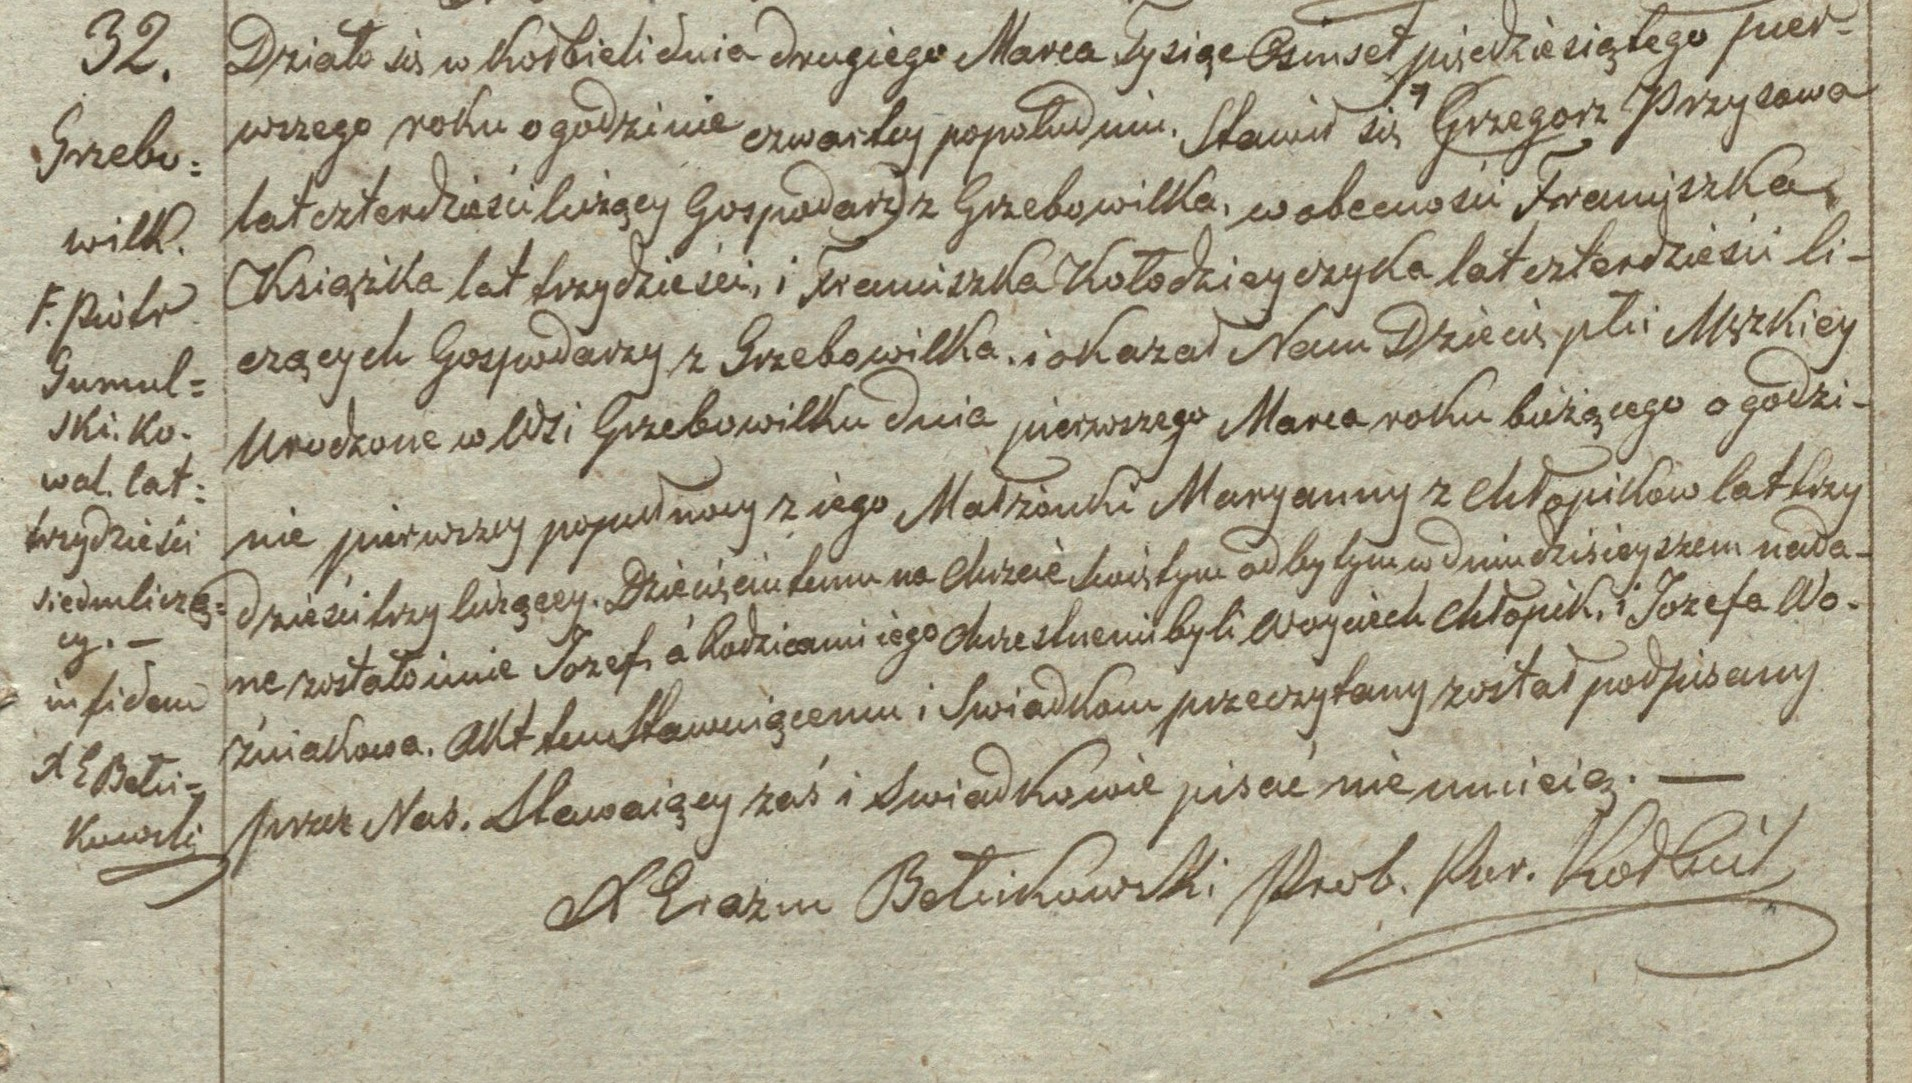
\includegraphics[width=1.0\linewidth]{
        1851_Józef_Gomulski_akt_chrztu_parafia_Kołbiel_wpis_32.jpg}
    \captionsetup{format=hang}
    \caption{Akt chrztu Józefa Gomulskiego - par. Kołbiel 1851~rok 
    (32/1851) \cite{par_kolbiel2}.}
    \label{fig:jgomulski_1851}
\end{figure}

\begin{figure}[!ht]
    \vspace*{0.5cm}
    \centering 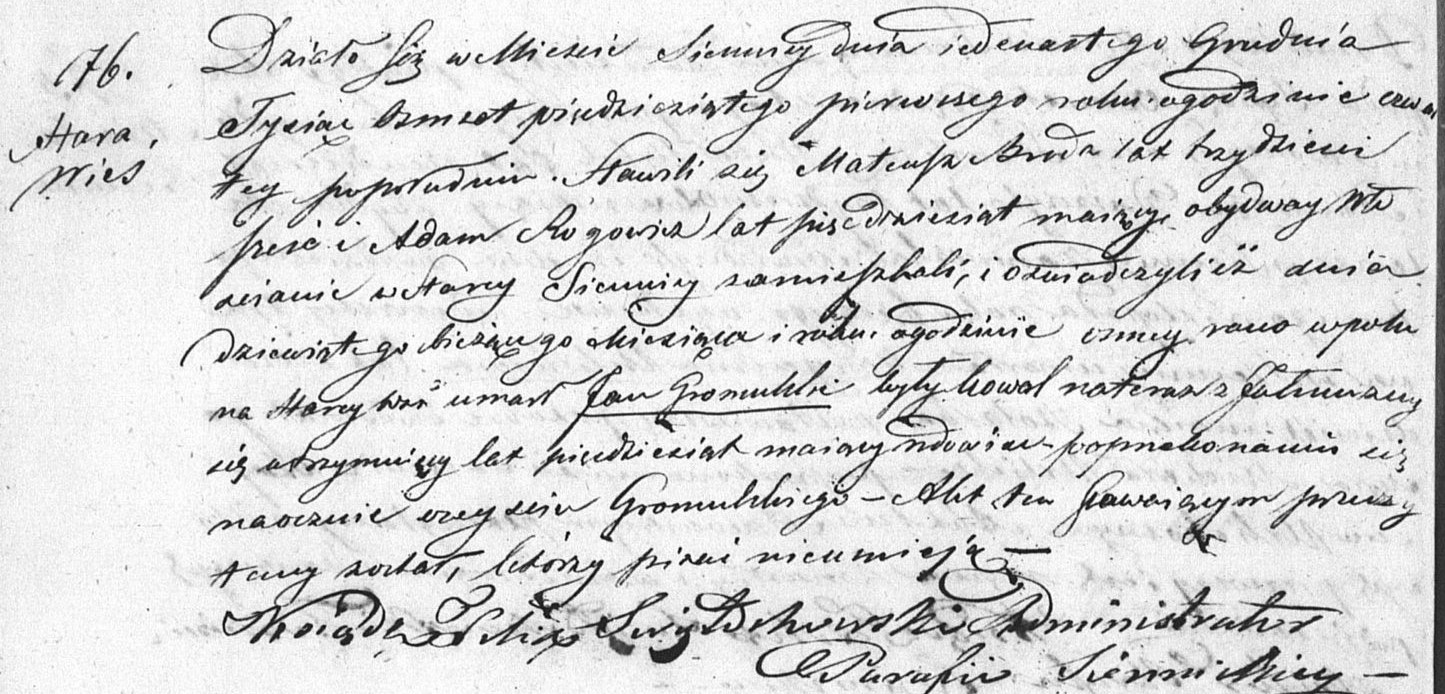
\includegraphics[width=1.0\linewidth]{
        1851_Jan_Gumulski_akt_zgonu_parafia_Siennica_wpis_76.jpg}
    \captionsetup{format=hang}
    \caption{Akt zgonu Jana Gomoły - par. Siennica 1851~rok 
    (76/1851) \cite{par_siennica}.}
    \label{fig:jgomulski_1851}
\end{figure}

Na przełomie 1851 oraz 1852~roku umierają rodzice Piotra Franciszka 
Gumulskiego, którzy prawdopodobnie, przynajmniej przez jakiś czas, mieszkali 
z~jego rodziną w~Grzebowilku. Pierwszy umiera jego ojciec Jan Gomoła - jego 
zgon we wsi Stara Wieś pod Siennicą (oddalonej od Grzebowilka o~około 
7~kilometrów) zgłaszają Mateusz Broda oraz Adam Rogowicz (patrz: ryc. 
\ref{fig:jgomulski_1851}). W~akcie swojego zgonu Jan Gomoła został określony 
jako \enquote{...Jan Gromulski były kowal na teraz z~jałmużny się 
utrzymujący...}. Prawdopodobnie nie mając już sił by pracować 
jako kowal i~nie chcąc być ciężarem dla rodziny, Jan Gomoła zdecydował się 
zostać wędrownym żebrakiem (dziadem). \textbf{Dnia 9~grudnia 1851~roku, po 
ponad 62~latach życia, zakończyła się historia Jana Gomoły vel Sokoła vel 
Gumuła vel Gumulskiego vel Gomulskiego vel Gromulskiego, założyciela rodziny 
Gomulskich.} Nieco ponad miesiąc po jego śmierci, 26~stycznia 1852~roku 
w~Grzebowilku zmarła jego żona Łucja Gomoła z~domu Rokicka. W~akcie jej zgonu 
wpisano \enquote{...zmarła Łucja Gumulska wdowa lat siedemdziesiąt licząca 
wyrobnica córka Wojciech i~Teresy małżonków Rokickich już zmarłych...} 
(patrz: ryc. \ref{fig:lgomola_1852}).

\begin{figure}[!ht]
    \vspace*{0.5cm}
    \centering 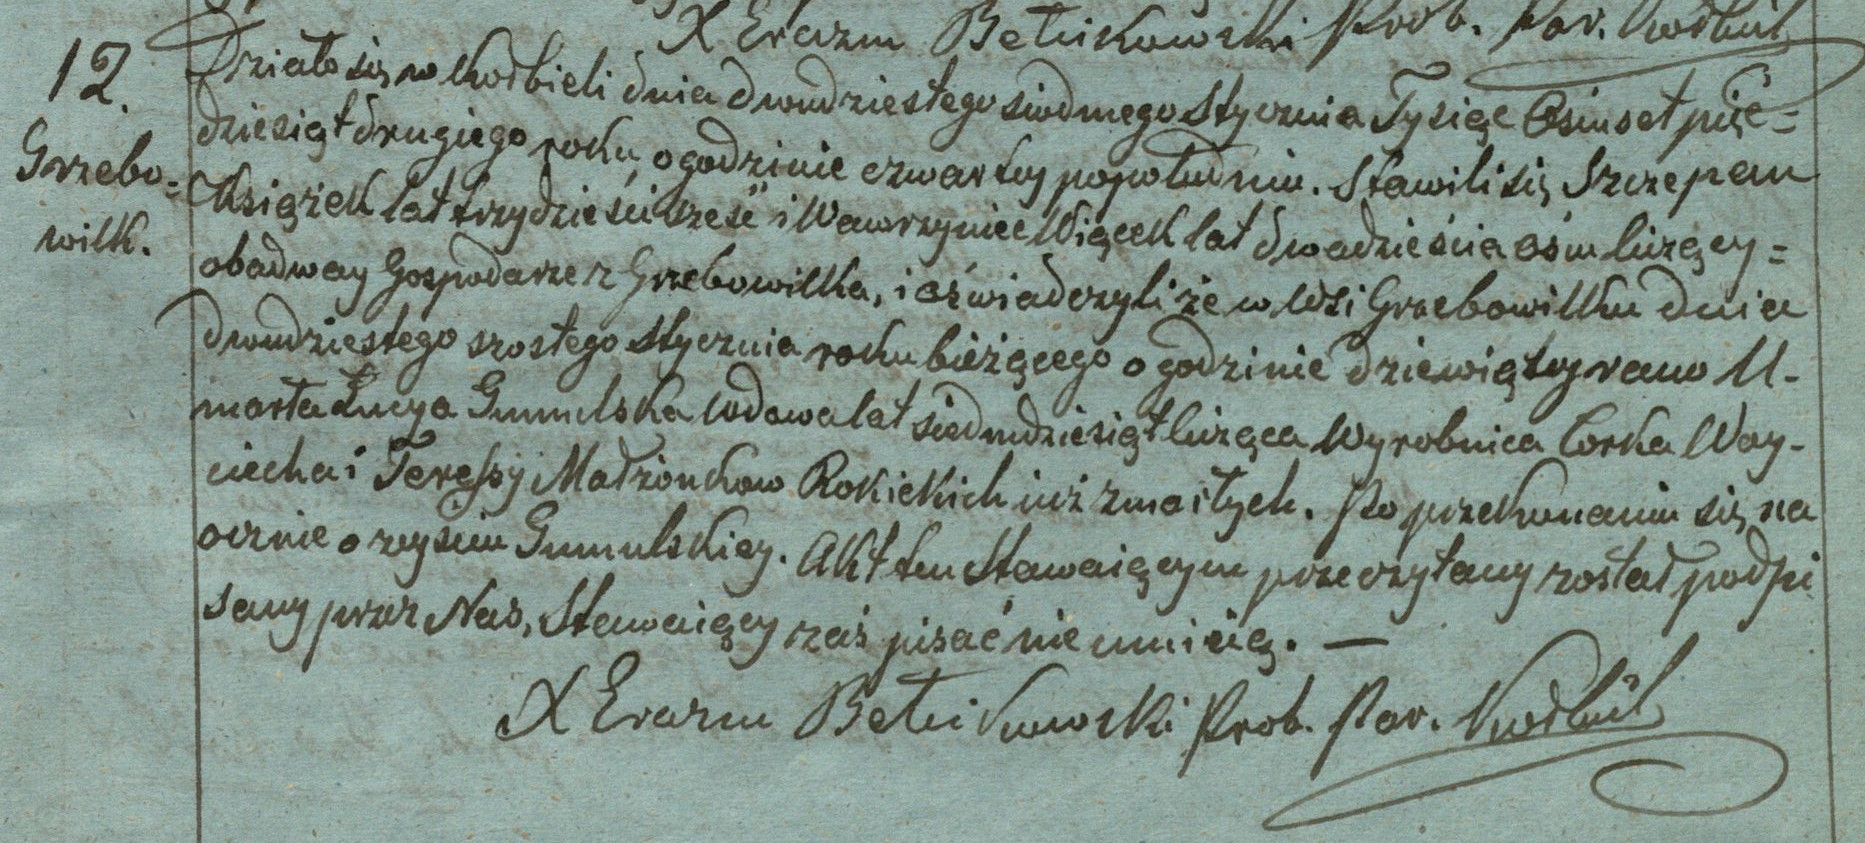
\includegraphics[width=1.0\linewidth]{
        1852_Łucja_Gomulska_Rokicka_akt_zgonu_parafia_Kołbiel_wpis_12.jpg}
    \captionsetup{format=hang}
    \caption{Akt zgonu Łucji Gomoły - par. Kołbiel 1852~rok (12/1852) 
    \cite{par_kolbiel2}.}
    \label{fig:lgomola_1852}
\end{figure}

Prawodopodobnie niedługo po śmierci swojej matki, Piotr Franciszek Gumulski 
wraz z~żoną, piątką dzieci oraz swoim młodszym, dwudziestokilkuletnim bratem 
Andrzejem opuścili wieś Grzebowilk by przeprowadzić się do oddalonej o~około 
siedem kilometrów na północny wschód Anieliny.

\clearpage
\textbf{\large Podsumowanie najważniejszych informacji o~członkach rodziny 
Gumulskich z~Rudzienka, Zamienia i~Grzebowilka}

\begin{figure}[!ht]
    \vspace*{0.5cm}
    \centering \includegraphics[width=0.85\linewidth]{Jan_Gomoła_karta.png}
\end{figure}

\begin{figure}[!ht]
    \vspace*{0.5cm}
    \centering 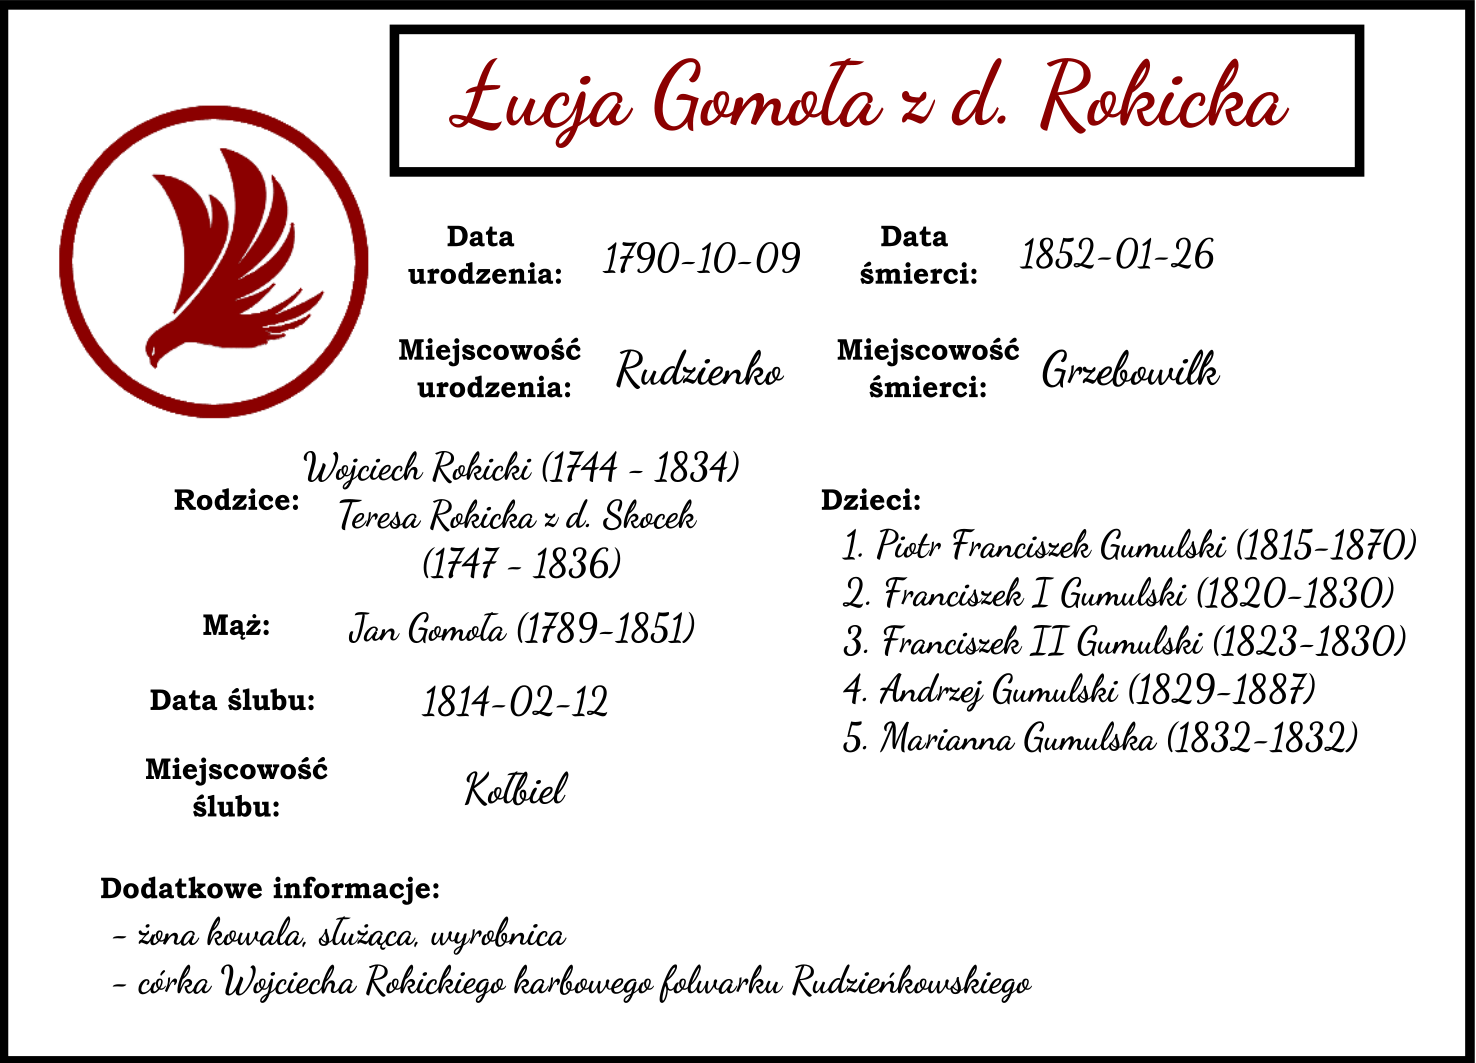
\includegraphics[width=0.85\linewidth]{Łucja_Gomoła_karta.png}
\end{figure}

\begin{figure}[!ht]
    \vspace*{0.5cm}
    \centering \includegraphics[width=0.65\linewidth]{
        Anna_Gomoła_karta.png}
\end{figure}

\begin{figure}[!ht]
    \vspace*{0.5cm}
    \centering 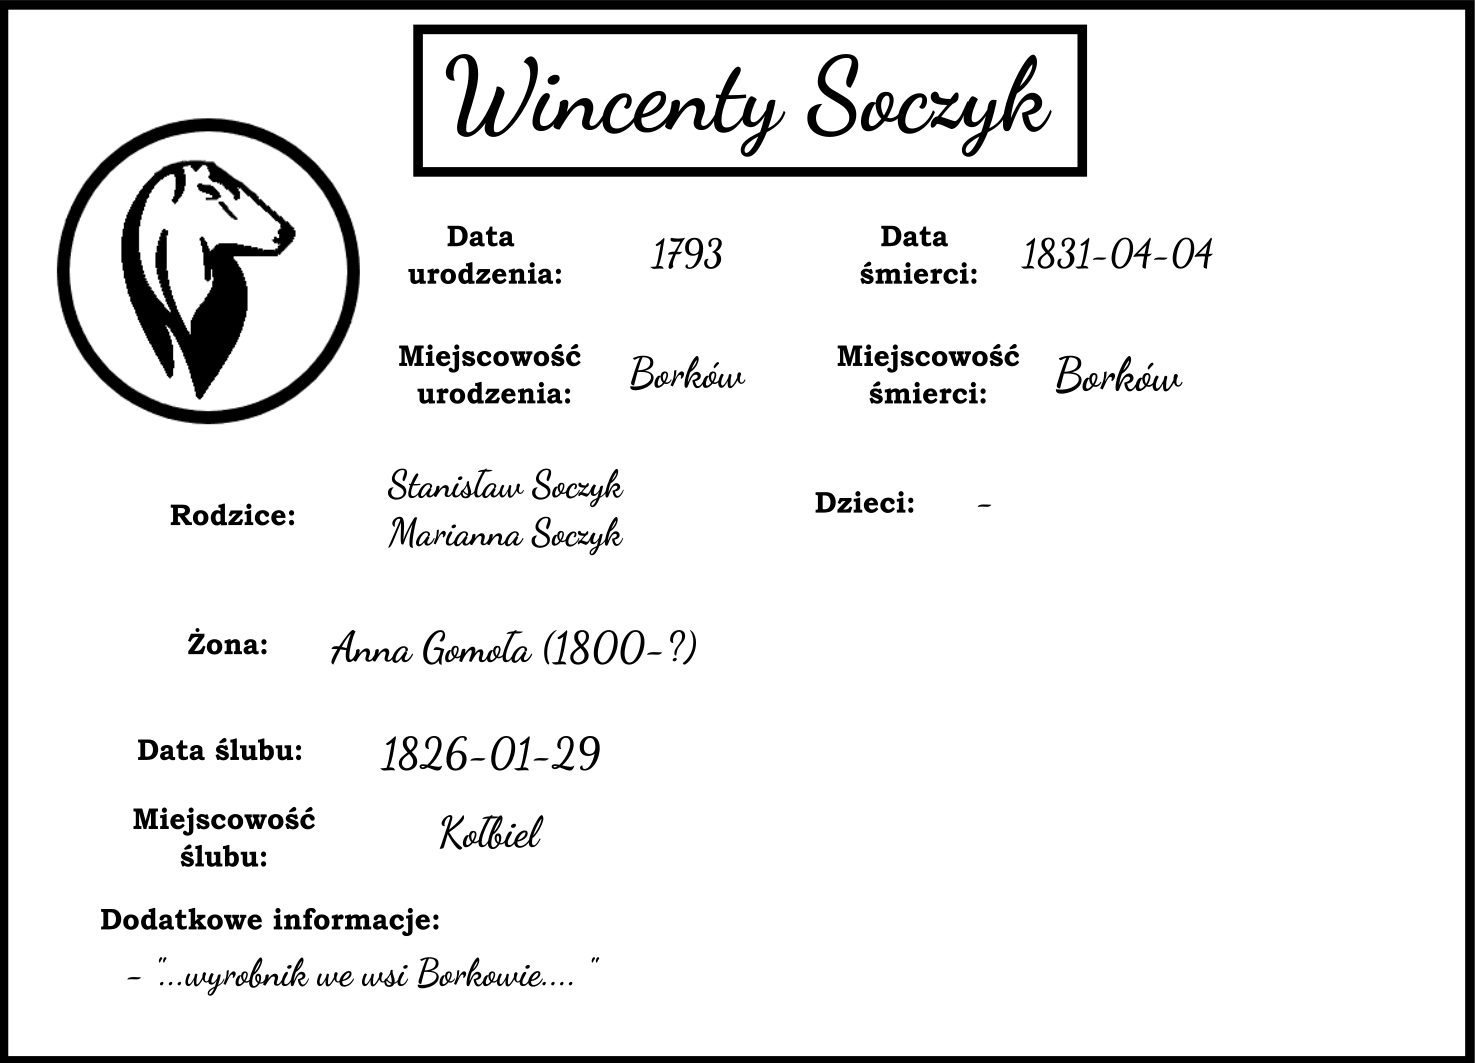
\includegraphics[width=0.65\linewidth]{
        Wincenty_Soczyk_karta.png}
\end{figure}

\begin{figure}[!ht]
    \vspace*{0.5cm}
    \centering 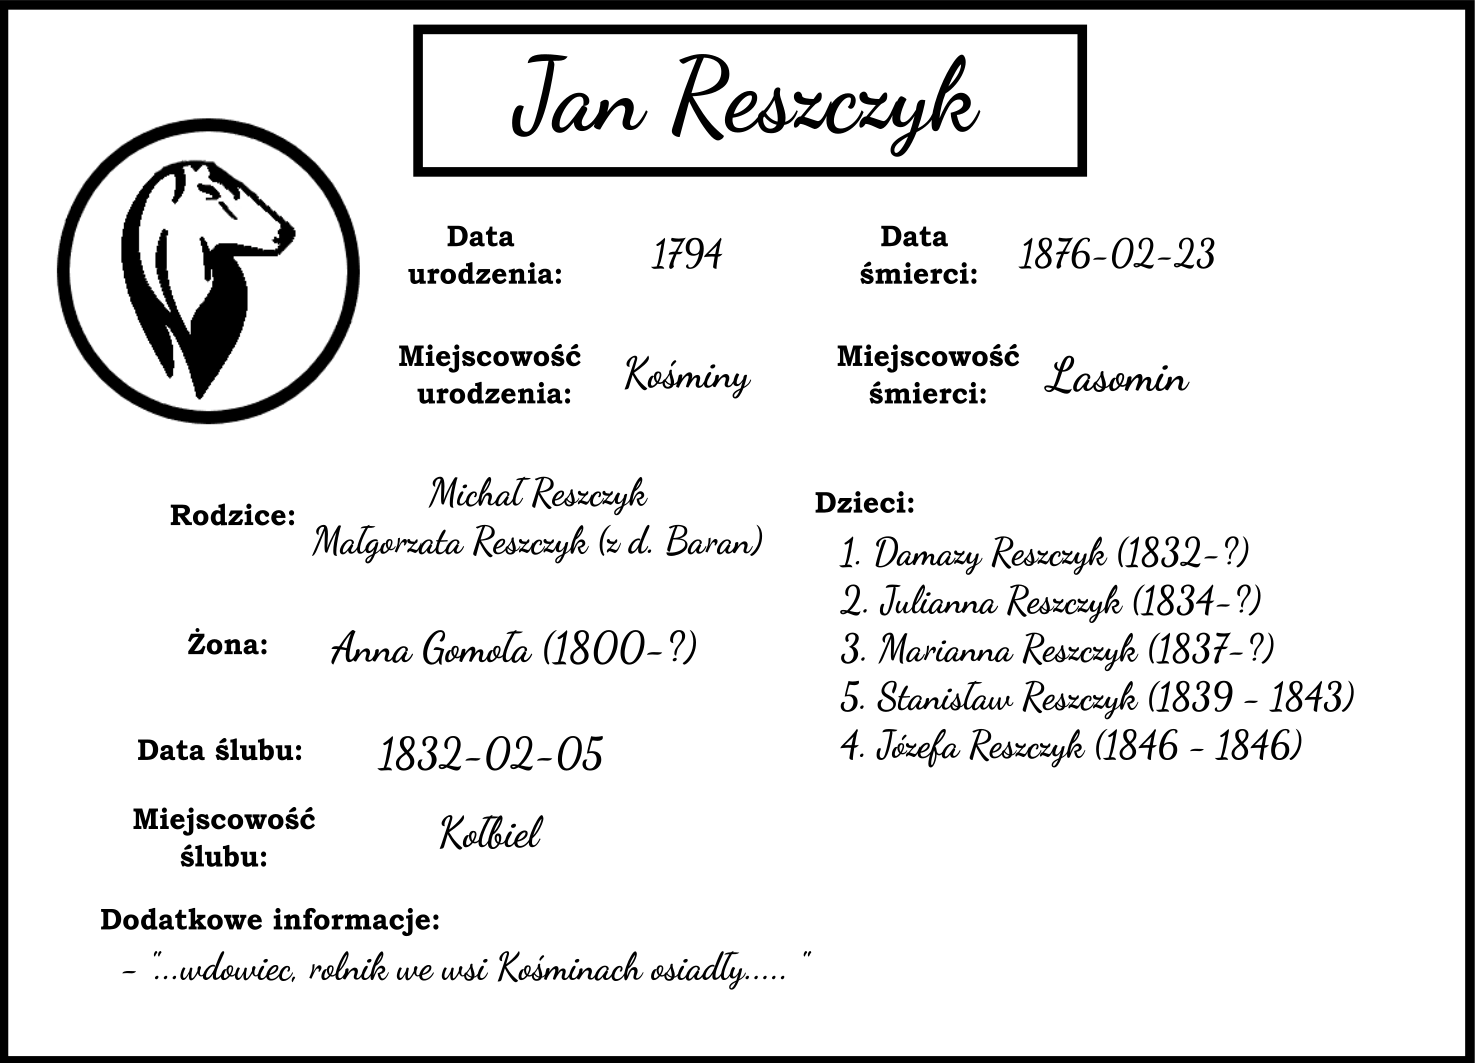
\includegraphics[width=0.65\linewidth]{
        Jan_Reszczyk_karta.png}
\end{figure}

\begin{figure}[!ht]
    \vspace*{0.5cm}
    \centering 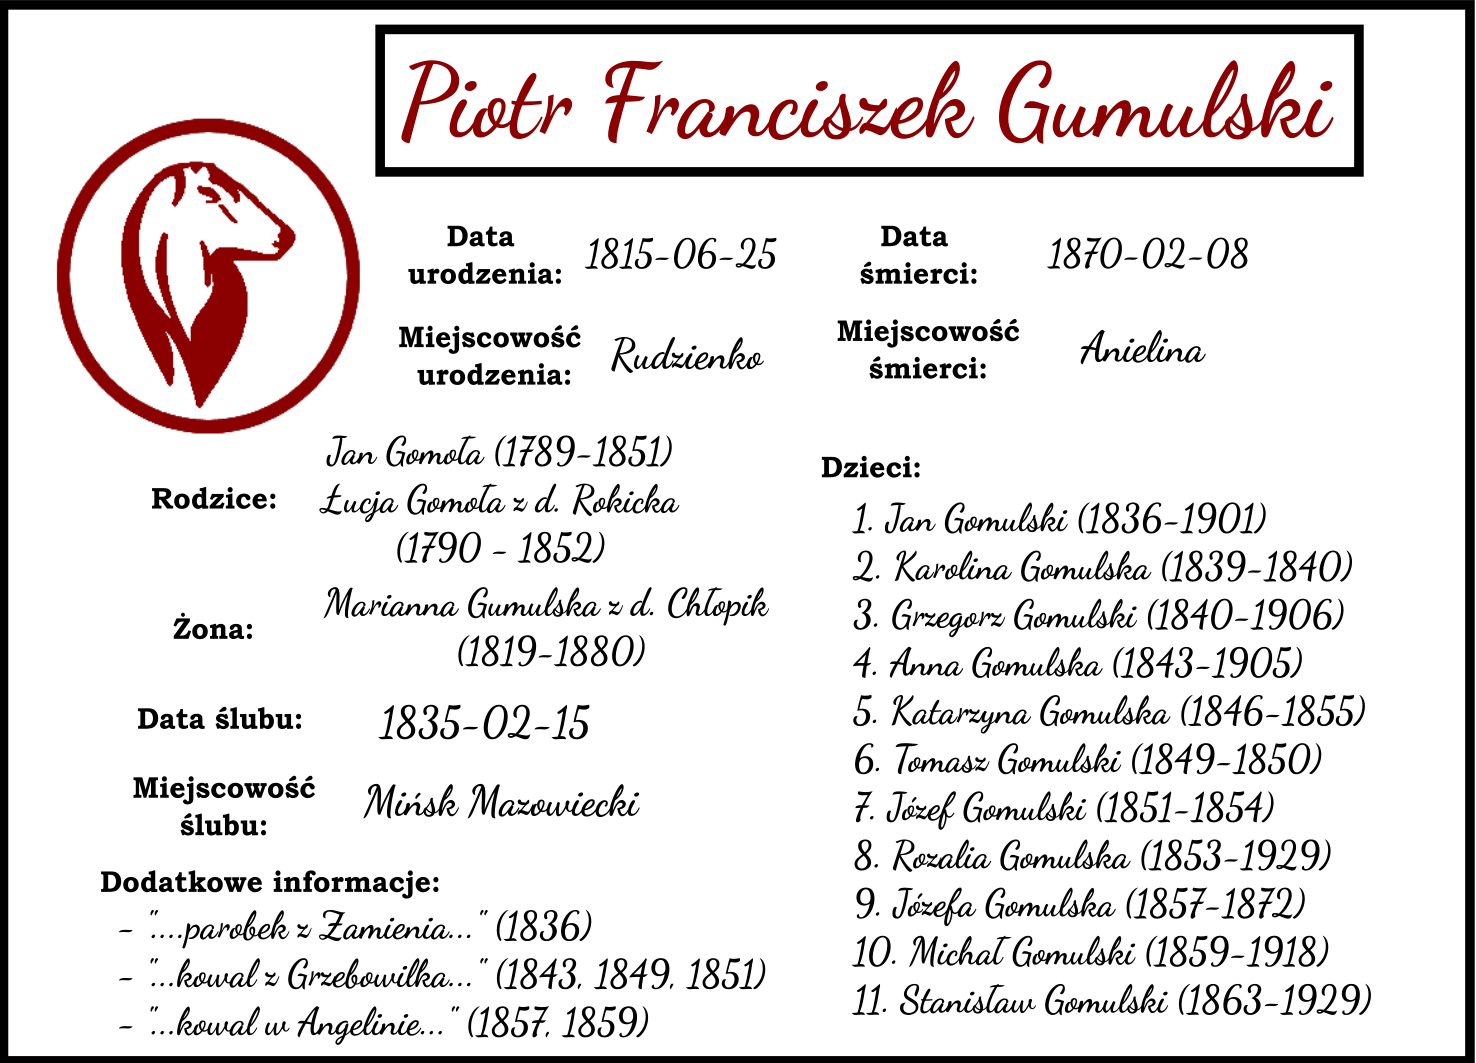
\includegraphics[width=0.85\linewidth]{
        Piotr_Franciszek_Gumulski_karta.png}
\end{figure}

\begin{figure}[!ht]
    \vspace*{0.5cm}
    \centering 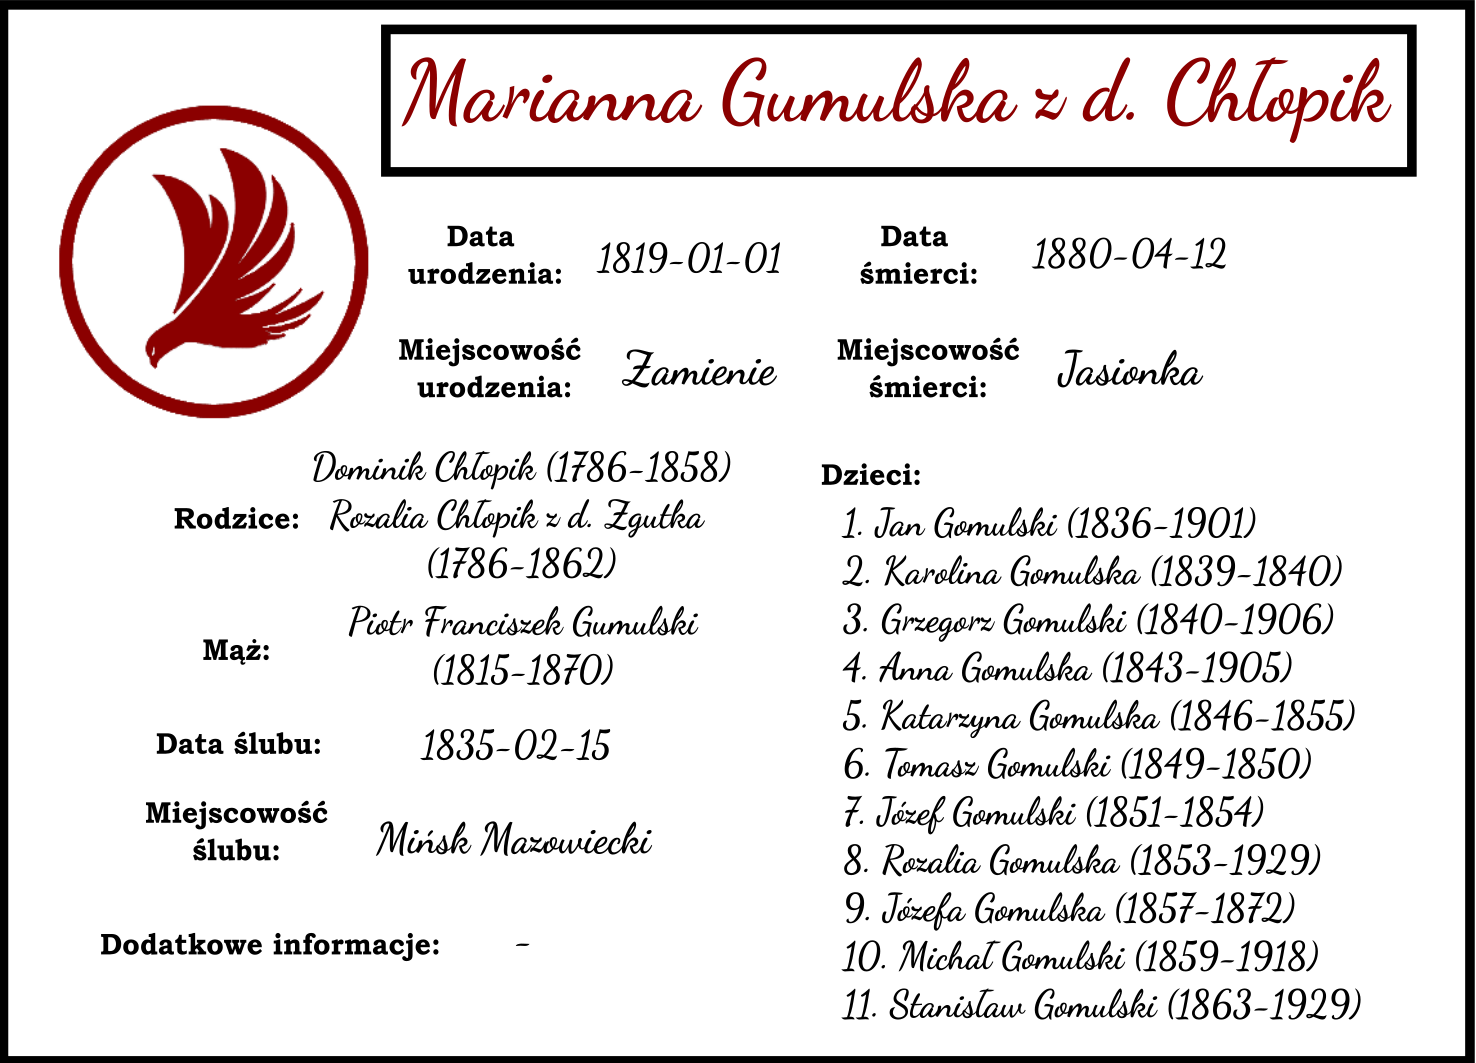
\includegraphics[width=0.85\linewidth]{
        Marianna_Gumulska_1819_karta.png}
\end{figure}

\begin{figure}[!ht]
    \vspace*{0.5cm}
    \centering 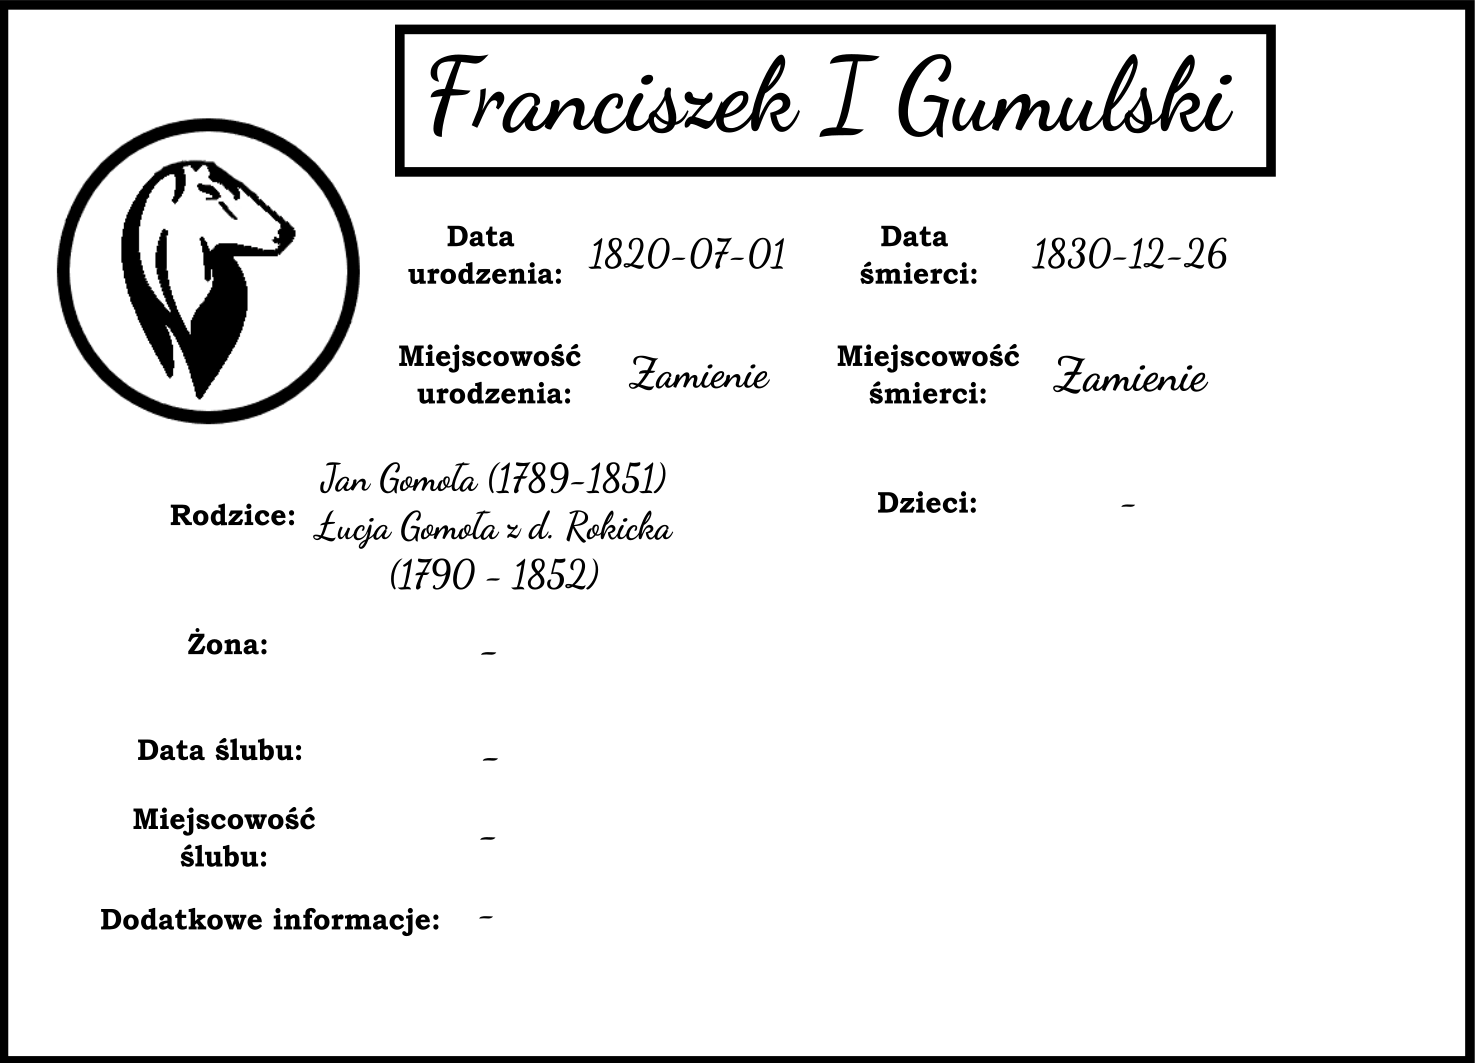
\includegraphics[width=0.65\linewidth]{
        Franciszek_I_Gumulski.png}
\end{figure}

\begin{figure}[!ht]
    \vspace*{0.5cm}
    \centering 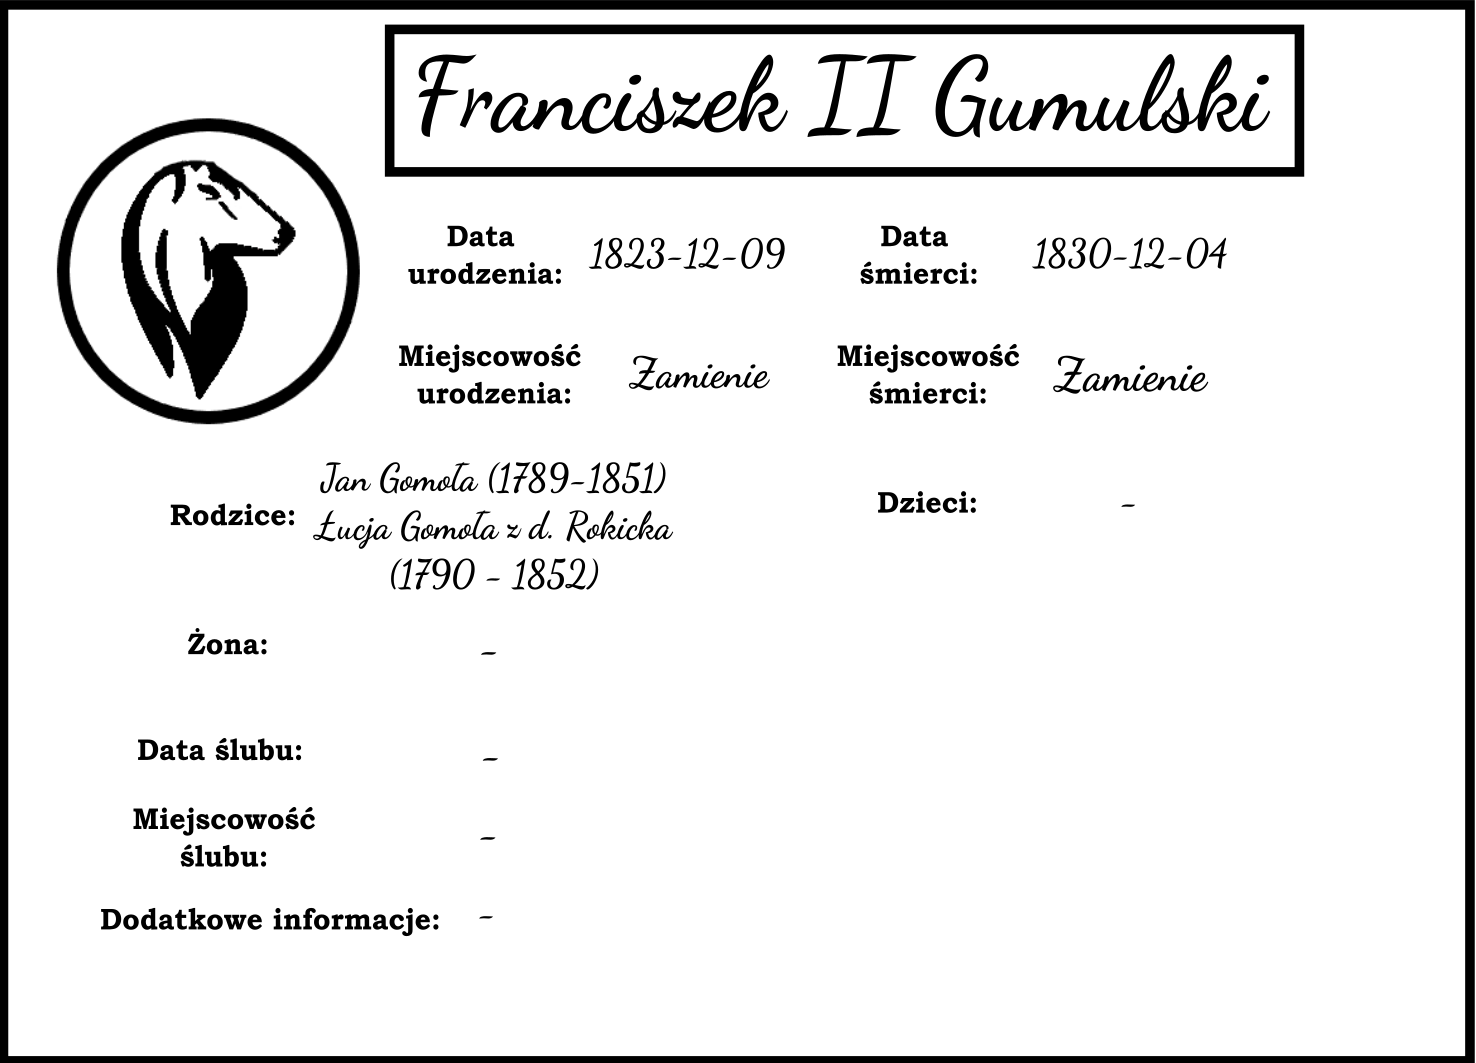
\includegraphics[width=0.65\linewidth]{
        Franciszek_II_Gumulski.png}
\end{figure}

\begin{figure}[!ht]
    \vspace*{0.5cm}
    \centering 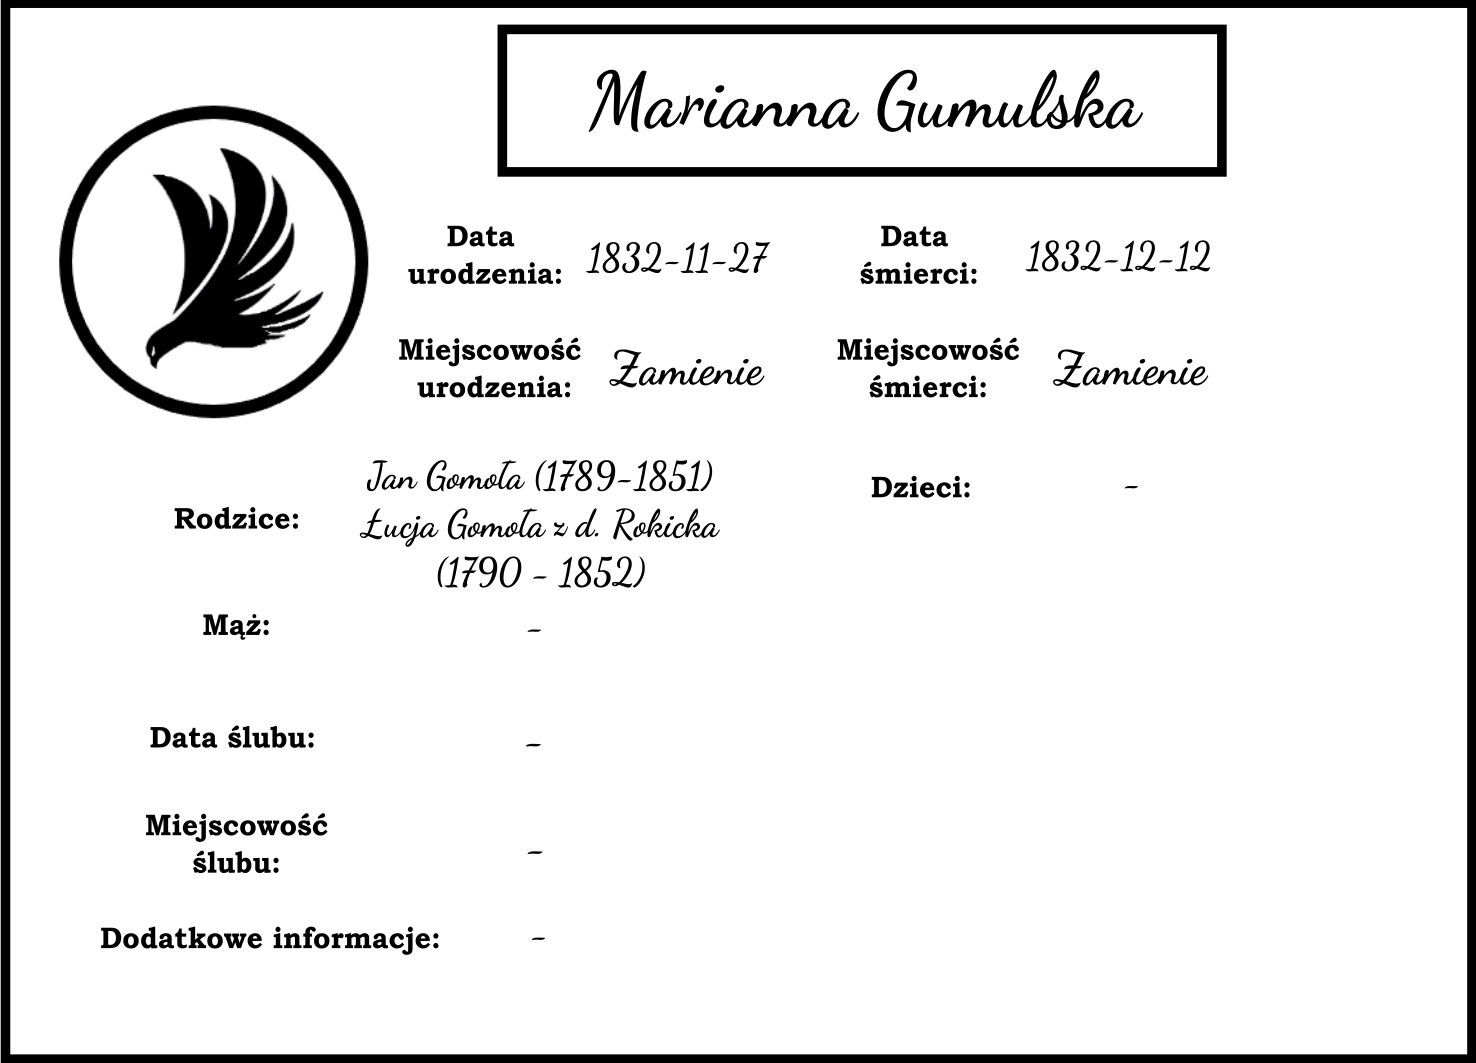
\includegraphics[width=0.65\linewidth]{
        Marianna_Gumulska_1832_karta.png}
\end{figure}

\begin{figure}[!ht]
    \vspace*{0.5cm}
    \centering 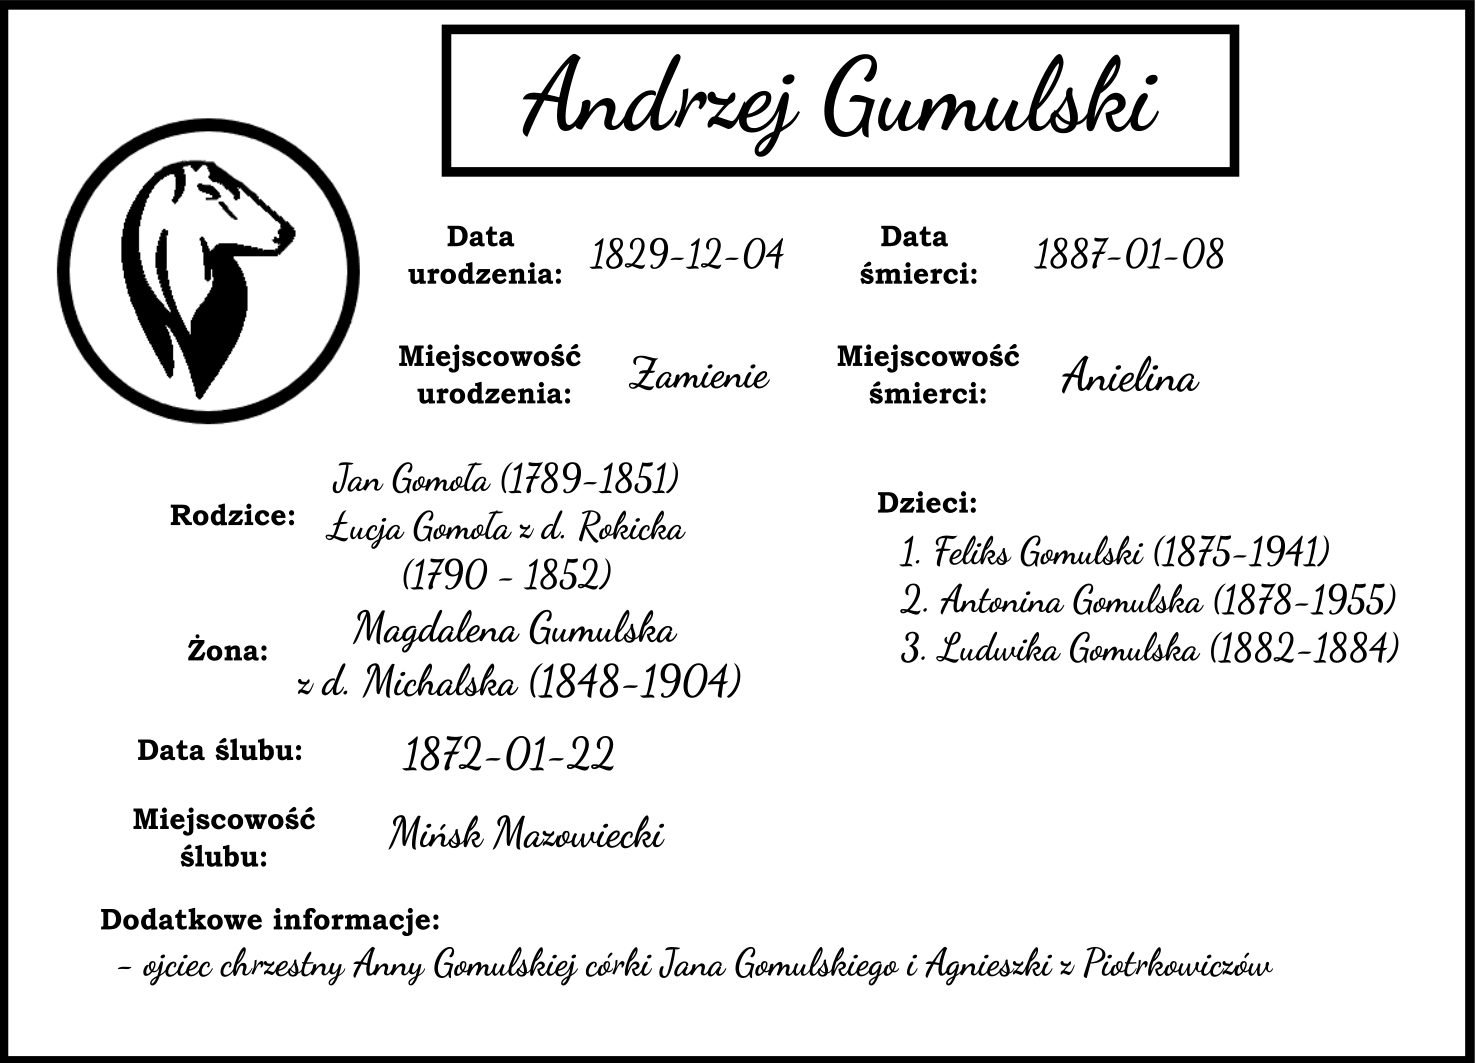
\includegraphics[width=0.85\linewidth]{
        Andrzej_Gumulski_karta.png}
\end{figure}

\begin{figure}[!ht]
    \vspace*{0.5cm}
    \centering 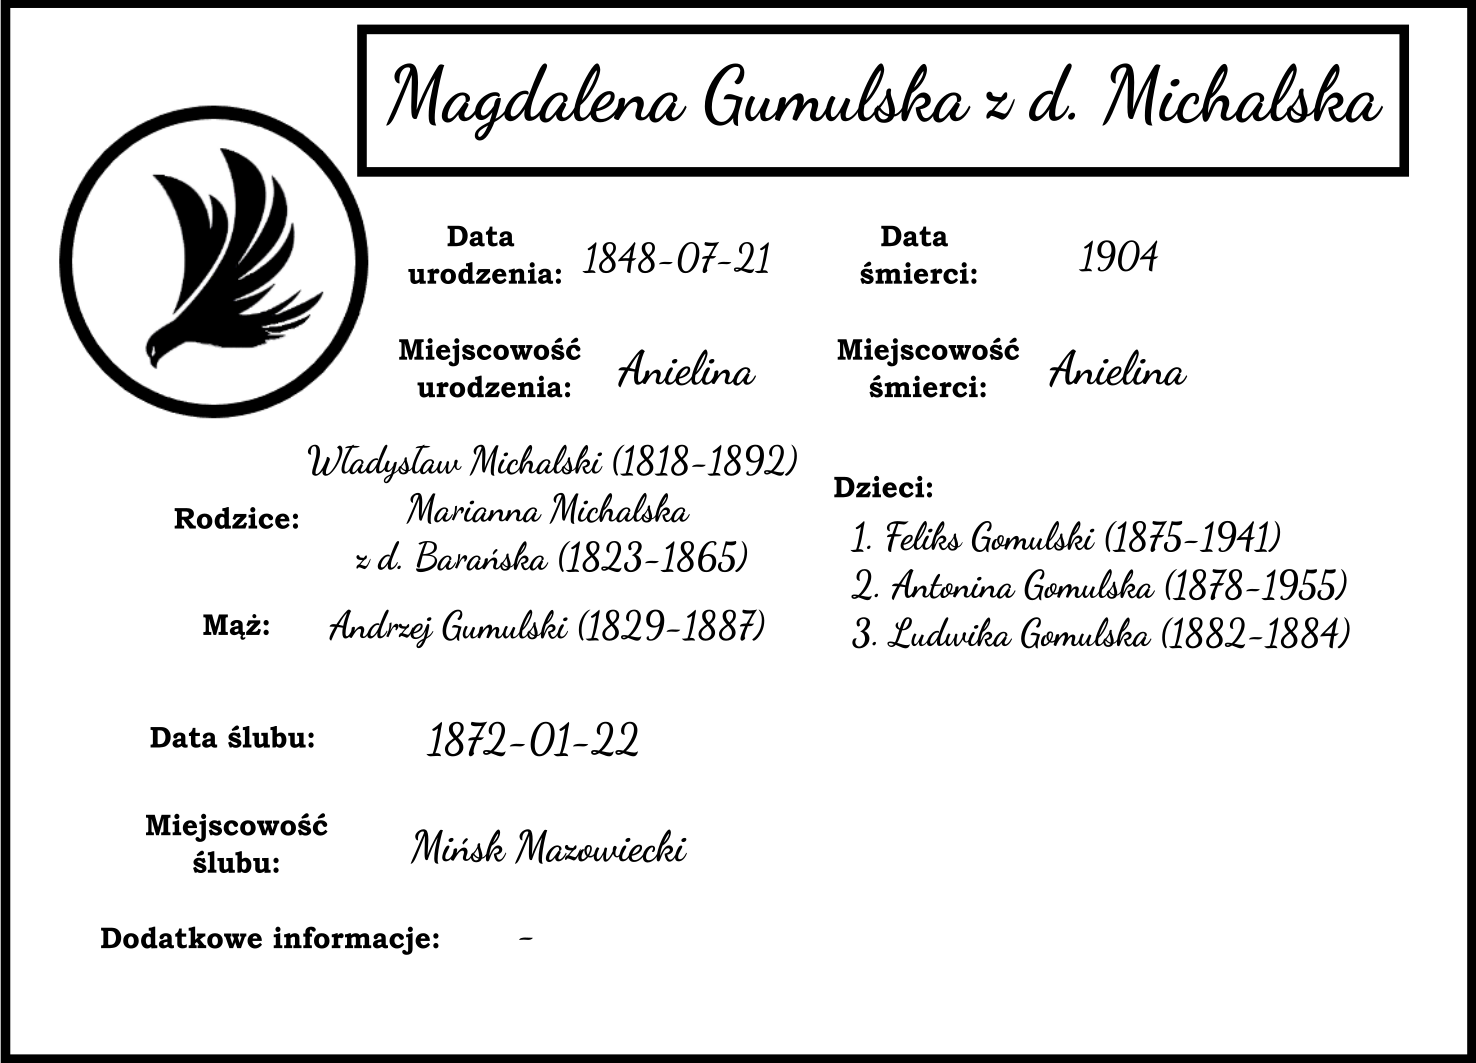
\includegraphics[width=0.85\linewidth]{
        Magdalena_Gumulska_karta.png}
\end{figure}

\begin{sidewaysfigure}
    \centering \includegraphics[width=1.0\linewidth]{
        Drzewo - Pokolenie I-III.png}
    \captionsetup{format=hang}
    \caption{Drzewo genealogiczne rodziny Gomulskich - Pokolenia I-III.}
\end{sidewaysfigure}